\documentclass[11pt]{article}

\usepackage[utf8]{inputenc}
\usepackage[T1]{fontenc}
\usepackage[spanish,es-tabla]{babel}

% Fuente y mejor espaciado
\usepackage{lmodern}
\usepackage{microtype}

\usepackage{geometry}
\usepackage{graphicx}
\usepackage{float}
\usepackage{subcaption}
\usepackage{amsmath}
\usepackage{amssymb}
\usepackage{amsfonts}
\usepackage{booktabs}
\usepackage{array}
\usepackage[table,xcdraw]{xcolor}
\usepackage{adjustbox}
\usepackage{listings}
\usepackage{url}
\usepackage{cite}
\usepackage{hyperref}
\usepackage{fancyhdr}
\usepackage{pifont}
\IfFileExists{dsfont.sty}{\usepackage{dsfont}}{}
\IfFileExists{bbm.sty}{\usepackage{bbm}}{}

\geometry{bottom=3cm, top=3cm, left=3cm, right=3cm}
\setlength{\parskip}{0.55em}
\setlength{\parindent}{0pt}
\setlength{\headheight}{15pt}
\renewcommand{\arraystretch}{1.25}
\graphicspath{{./}{../}{../figs/}}

\definecolor{myblue}{RGB}{0,0,128}
\definecolor{myred}{RGB}{128,0,0}
\definecolor{mygreen}{RGB}{0,128,0}

\hypersetup{
    colorlinks=true,
    linkcolor=myblue,
    citecolor=myred,
    filecolor=magenta,
    urlcolor=cyan
}

\renewcommand{\sectionautorefname}{Secci\'on}
\renewcommand{\subsectionautorefname}{Subsecci\'on}
\renewcommand{\subsubsectionautorefname}{Subsubsecci\'on}
\renewcommand{\equationautorefname}{Ecuaci\'on}
\renewcommand{\figureautorefname}{Figura}
\renewcommand{\tableautorefname}{Tabla}
\addto\captionsspanish{\renewcommand{\tablename}{Tabla}}

\pagestyle{fancy}
\fancyhf{}
\fancyhead[L]{\nouppercase{\leftmark}}
\fancyfoot[L]{\textit{Informe de Proyecto}}
\fancyfoot[C]{\thepage}
\fancyfoot[R]{\textit{EL7007-1}}
\renewcommand{\headrulewidth}{0.4pt}
\renewcommand{\footrulewidth}{0.4pt}

\newcommand{\rankone}{\textit{Rank-1}}
\newcommand{\accglobal}{\texttt{accuracy\_global}}
\newcommand{\detectorinput}{\texttt{det\_size}}

\begin{document}

\hypersetup{pageanchor=false}
\begin{titlepage}
\centering
{\includegraphics[width=0.78\textwidth]{\detokenize{Portada/logo die (1) (1) (3) (1) (2) (2).png}}}
\vspace{1cm}

{\scshape\Large EL7007-1 Introducci\'on al Procesamiento Digital de Im\'agenes \par}
\vspace{2.7cm}

{\scshape\Huge Informe de Proyecto\par}
\vspace{0.5cm}
{\scshape\Large Reconocimiento de rostros desde drones\par}
\vspace{3.7cm}

\begin{flushright}
{\large Autores: Mart\'in Aburto y Fernando Quintero\par}
\vspace{0.5cm}
{\large Profesor: Claudio P\'erez Flores\par}
\vspace{0.5cm}
{\large Auxiliar: Christian D\'iaz Guerra\par}
\vspace{0.5cm}
{\large Ayudante: Renato Cariaga C\'arcamo\par}
\vspace{0.5cm}
{\large Ayudante de Laboratorio: Juan Pablo P\'erez Caballero\par}
\vspace{0.5cm}
{\large \today \par}
\end{flushright}
\end{titlepage}

\clearpage
\hypersetup{pageanchor=true}
\pagenumbering{arabic}
\setcounter{page}{1}



\renewcommand{\contentsname}{Índice general}
\renewcommand{\listtablename}{Índice de tablas}
\renewcommand{\listfigurename}{Índice de figuras}

\tableofcontents
\clearpage

\phantomsection
\addcontentsline{toc}{section}{\listtablename}
\listoftables
\clearpage

\phantomsection
\addcontentsline{toc}{section}{\listfigurename}
\listoffigures



\newpage

\section{Introducci\'on}
\label{sec:introduccion}

El reconocimiento facial en im\'agenes capturadas desde drones es un problema m\'as exigente que el reconocimiento en fotograf\'ias frontales controladas. La distancia entre la c\'amara y el sujeto reduce la resoluci\'on efectiva del rostro; adem\'as, la altura, el \'angulo de captura, la compresi\'on y el desenfoque afectan tanto la detecci\'on facial como la calidad del descriptor extra\'ido. Por esto, evaluar un sistema solamente con rostros ya recortados puede entregar una estimaci\'on optimista del desempe\~no real.

Este proyecto implementa un flujo reproducible sobre DroneFace \cite{hsu2017droneface}, usando InsightFace con el paquete preentrenado \texttt{buffalo\_l}. El sistema no entrena una red desde cero y no implementa control de dron; el foco est\'a en medir el desempe\~no de un pipeline de detecci\'on y reconocimiento facial sobre im\'agenes con condiciones cercanas a captura a\'erea. El reconocedor genera embeddings tipo ArcFace \cite{deng2019arcface}, los cuales se comparan mediante similitud coseno contra una galer\'ia de identidades conocidas.

La versi\'on final del proyecto corrige una limitaci\'on del baseline preliminar: en vez de usar solamente \texttt{portraits}, se construyen galer\'ias desde \texttt{trio\_cam} y \texttt{trio\_gp}. Esto permite incluir los 11 sujetos de DroneFace en la galer\'ia y evaluar todos los recortes de \texttt{photos\_all\_faces}, sin excluir identidades por falta de referencia. Adem\'as, se agrega una evaluaci\'on a nivel de cajas delimitadoras (\textit{bbox-level}) usando anotaciones manuales del orden espacial de los sujetos en las im\'agenes completas.

El informe se organiza en tres experimentos y un protocolo complementario:

\begin{itemize}
    \item \textbf{Experimento A:} reconocimiento \textit{closed-set} sobre rostros recortados de \texttt{photos\_all\_\allowbreak faces}.
    \item \textbf{Experimento B:} recuperaci\'on de identidades esperadas en im\'agenes completas de \texttt{photos\_all}, usando supervisi\'on d\'ebil a nivel de conjunto.
    \item \textbf{Experimento C:} evaluaci\'on \textit{bbox-level} con asignaci\'on espacial manual de identidades esperadas.
    \item \textbf{Protocolo complementario:} verificaci\'on por scores, curvas ROC/AUC y decisi\'on con \texttt{None}/\textit{unknown}.
\end{itemize}

Adem\'as, se comparan los resultados finales con dos referencias: la versi\'on V1 del propio proyecto, guardada en la carpeta \texttt{outputs/}, y el paper \textit{Face Recognition on Drones: Issues and Limitations} de Hsu y Chen \cite{hsu2015issues}, que estudia detecci\'on y reconocimiento facial en un escenario de dron con Face++, ReKognition y detectores cl\'asicos de OpenCV.

\section{Marco te\'orico}
\label{sec:marco}

\subsection{Reconocimiento facial con embeddings}

Los sistemas modernos de reconocimiento facial suelen representar cada rostro mediante un vector num\'erico llamado \textit{embedding}. La idea central es que dos im\'agenes de la misma persona deben quedar cercanas en el espacio de embeddings, mientras que identidades distintas deben quedar separadas. Este enfoque aparece en modelos como FaceNet \cite{schroff2015facenet} y ArcFace \cite{deng2019arcface}.

En este proyecto se usa identificaci\'on \textit{closed-set}: cada rostro evaluado pertenece a una identidad presente en la galer\'ia. Dado un embedding de prueba $\mathbf{x}$ y una galer\'ia de embeddings $\{\mathbf{g}_i\}$, la similitud se calcula mediante coseno:

\begin{equation}
    \operatorname{sim}(\mathbf{x}, \mathbf{g}_i)
    =
    \frac{\mathbf{x}^{T}\mathbf{g}_i}{\|\mathbf{x}\|_2\|\mathbf{g}_i\|_2}.
\end{equation}

La identidad predicha corresponde al vecino m\'as similar:

\begin{equation}
    \hat{y} =
    \arg\max_i \operatorname{sim}(\mathbf{x}, \mathbf{g}_i).
\end{equation}

En los experimentos \textit{closed-set} no se usa umbral de desconocido. Por lo tanto, si se detecta un rostro, el sistema siempre lo asigna a la identidad m\'as parecida dentro de la galer\'ia. El umbral \texttt{None}/\textit{unknown} se eval\'ua despu\'es como un protocolo complementario de verificaci\'on.

\subsection{ArcFace, InsightFace y detecci\'on facial}

ArcFace propone una p\'erdida con margen angular aditivo para obtener embeddings m\'as discriminativos \cite{deng2019arcface}. En este proyecto no se implementa ArcFace manualmente; se usa mediante InsightFace, una biblioteca que integra detecci\'on facial, alineamiento y extracci\'on de embeddings \cite{insightface2026}.

El paquete \texttt{buffalo\_l} de InsightFace combina submodelos diferentes. De acuerdo con el \textit{model zoo} de InsightFace, el paquete incluye un detector RetinaFace-10GF y un reconocedor ResNet50 entrenado sobre WebFace600K \cite{insightface_model_zoo}. El detector facial localiza cajas y puntos faciales; RetinaFace es un detector de una etapa dise\~nado para localizaci\'on facial y puntos de alineamiento \cite{deng2020retinaface}. Luego, el reconocedor produce el embedding usado para la comparaci\'on. En la ejecuci\'on local se usa el proveedor de CPU de ONNX Runtime, por lo que los resultados dependen del modelo preentrenado y de la configuraci\'on del detector, no de un proceso de entrenamiento propio.

El par\'ametro \detectorinput{} controla el tama\~no de entrada usado por el detector. Este par\'ametro no cambia la arquitectura del reconocedor ni reentrena el modelo, pero puede afectar la detecci\'on de rostros peque\~nos. En el pipeline V2 se mantuvo la configuraci\'on generada por el repositorio para las salidas finales.

\subsection{DroneFace}

DroneFace es un conjunto de datos dise\~nado para investigaci\'on con im\'agenes de dron \cite{hsu2017droneface}. En la copia local del proyecto se usan principalmente las carpetas:

\begin{itemize}
    \item \texttt{photos\_all\_faces}: rostros recortados con identidad conocida.
    \item \texttt{photos\_all}: im\'agenes completas con dos o tres personas.
    \item \texttt{trio\_cam} y \texttt{trio\_gp}: im\'agenes de referencia frontales y laterales para construir galer\'ias.
\end{itemize}

La \autoref{tab:droneface_summary} resume las condiciones principales reportadas para DroneFace. La copia local del dataset incluye una licencia ODbL/DbCL, por lo que en este informe se usan figuras generadas desde las im\'agenes locales y un esquema de la geometr\'ia de captura, en vez de reutilizar capturas de figuras de los trabajos originales.

\begin{table}[H]
\centering
\caption{Resumen del conjunto DroneFace usado como base experimental.}
\label{tab:droneface_summary}
\begin{adjustbox}{max width=\textwidth}
\begin{tabular}{ll}
\toprule
Caracter\'istica & Descripci\'on reportada \\
\midrule
Sujetos & 11 sujetos: 7 hombres y 4 mujeres \\
Volumen de datos & 2057 im\'agenes: 620 im\'agenes raw, 1364 rostros frontales recortados y 73 retratos \\
Captura raw & Resoluci\'on 3680$\times$2760, campo ultra amplio de 170$^\circ$ y luz diurna \\
Alturas & 1.5, 3, 4 y 5 m \\
Distancias & Entre 2 y 17 m, con intervalo de 0.5 m \\
Uso en este proyecto & Galer\'ias desde \texttt{trio\_cam}+\texttt{trio\_gp}; pruebas en \texttt{photos\_all\_faces} y \texttt{photos\_all} \\
\bottomrule
\end{tabular}
\end{adjustbox}
\end{table}

La \autoref{fig:droneface_geometry} muestra una recreaci\'on esquem\'atica de la configuraci\'on geom\'etrica del dataset. La idea relevante para este proyecto es que el aumento de altura y distancia reduce la resoluci\'on efectiva del rostro y cambia el \'angulo vertical de observaci\'on, lo que afecta primero a la detecci\'on y luego al reconocimiento.

\begin{figure}[H]
\centering
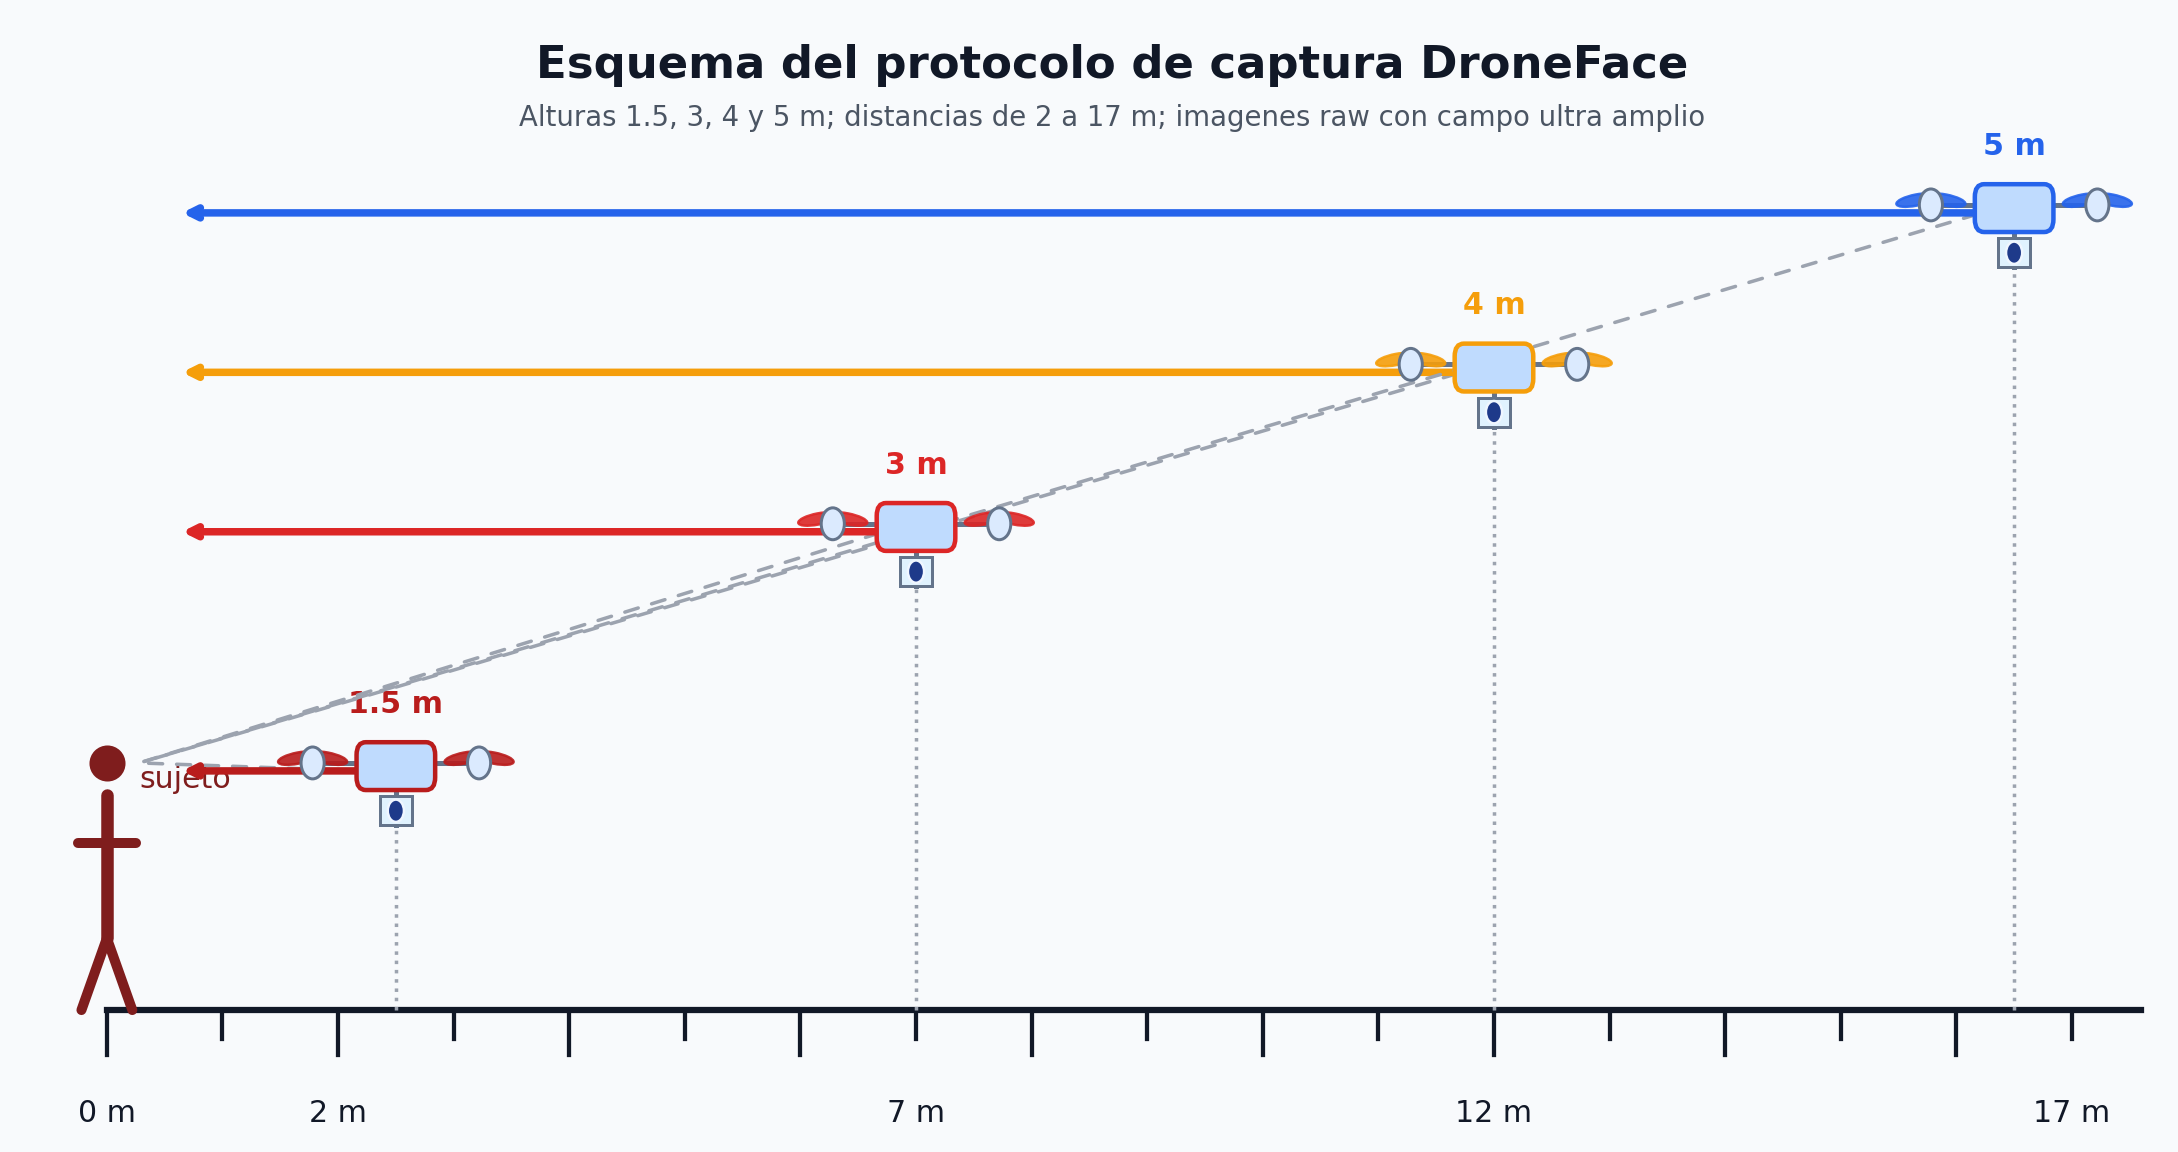
\includegraphics[width=0.96\textwidth]{figs/dataset/droneface_capture_geometry_schematic.png}
\caption{Esquema del protocolo de captura de DroneFace, basado en la descripci\'on del dataset.}
\label{fig:droneface_geometry}
\end{figure}

Para construir las galer\'ias se usaron las poses \texttt{porL}, \texttt{porF} y \texttt{porR} de \texttt{trio\_cam} y \texttt{trio\_gp}. La \autoref{fig:droneface_trio_examples} muestra ejemplos de dos sujetos en ambas fuentes de referencia. Estas im\'agenes explican por qu\'e se evaluaron tres galer\'ias: frontal, lateral y multi-pose.

\begin{figure}[H]
\centering
\begin{subfigure}[t]{0.49\textwidth}
    \centering
    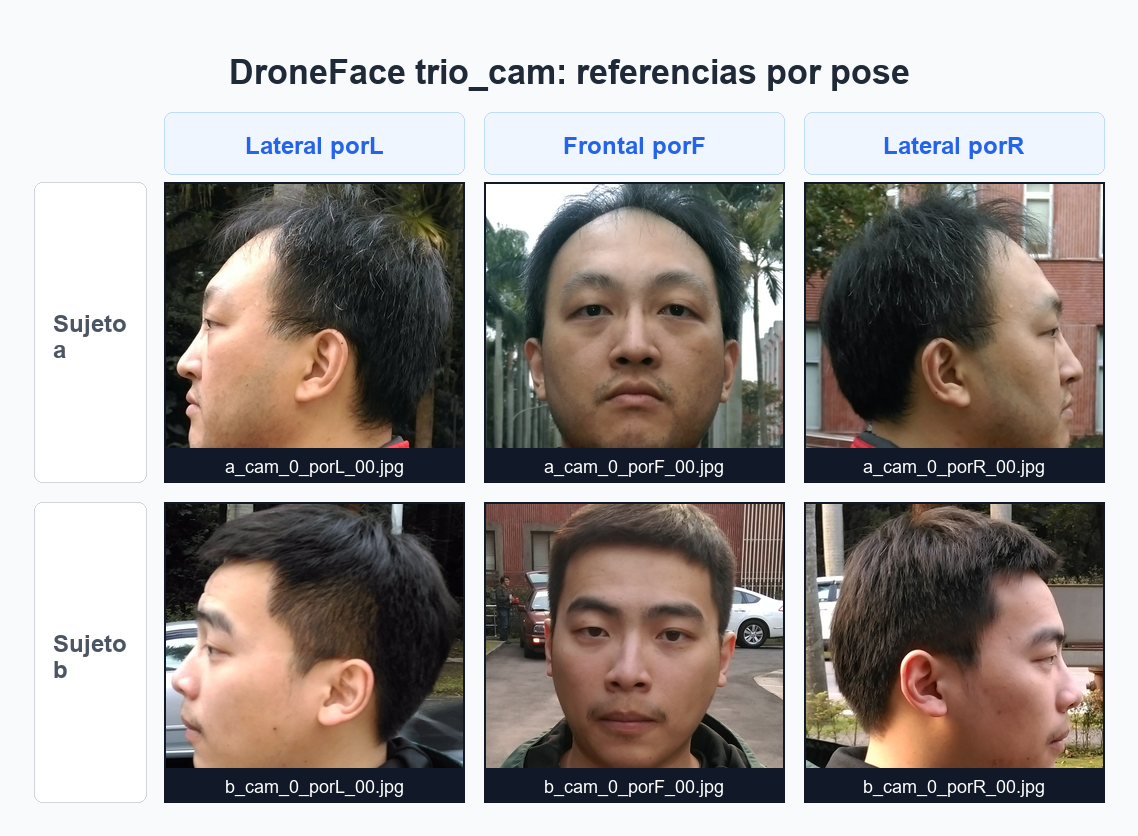
\includegraphics[width=\textwidth]{figs/dataset/droneface_trio_cam_pose_collage.png}
    \caption{\texttt{trio\_cam}.}
\end{subfigure}
\hfill
\begin{subfigure}[t]{0.49\textwidth}
    \centering
    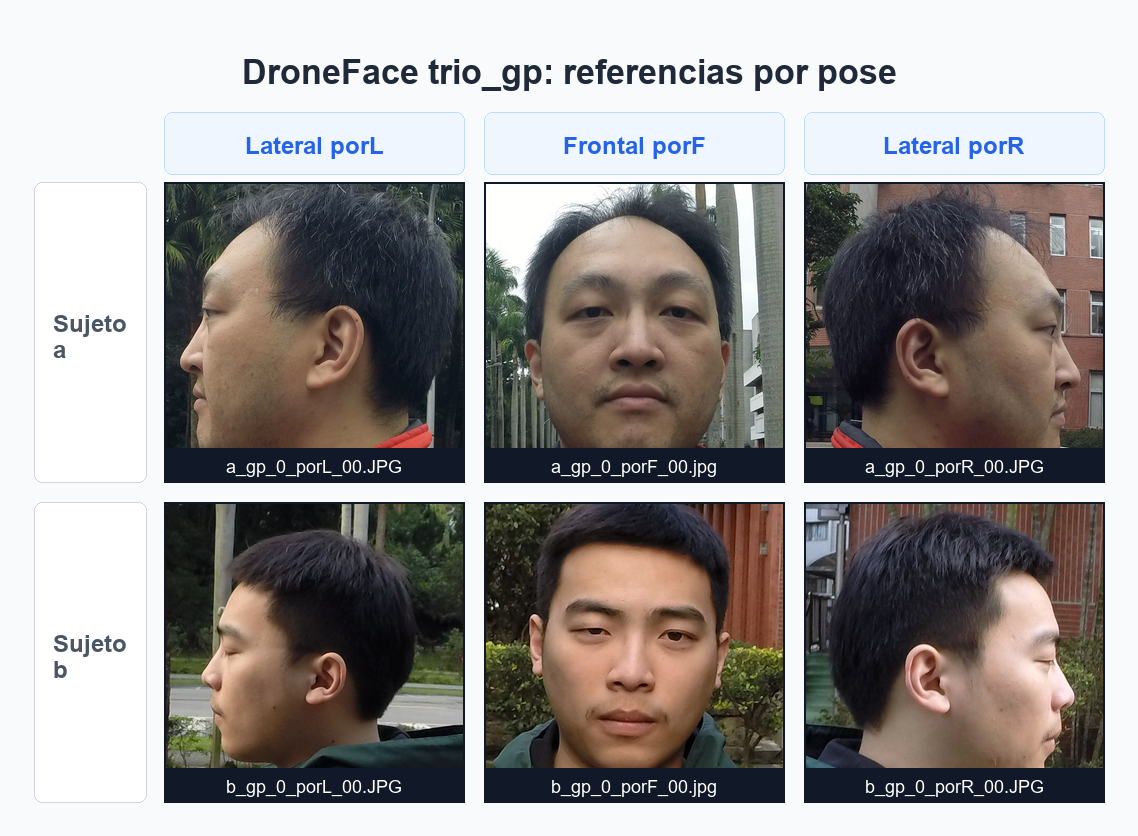
\includegraphics[width=\textwidth]{figs/dataset/droneface_trio_gp_pose_collage.png}
    \caption{\texttt{trio\_gp}.}
\end{subfigure}
\caption{Ejemplos propios de referencias por pose usadas para construir galer\'ias. Las columnas corresponden a \texttt{porL}, \texttt{porF} y \texttt{porR}.}
\label{fig:droneface_trio_examples}
\end{figure}

Las im\'agenes completas usan etiquetas compuestas como \texttt{ab}, \texttt{cd}, \texttt{ef}, \texttt{gh} e \texttt{ijk}. Estas etiquetas indican qu\'e sujetos aparecen en la imagen, pero no entregan por s\'i solas la identidad asociada a cada caja detectada. Por eso el proyecto separa la evaluaci\'on por conjunto de identidades esperadas y la evaluaci\'on \textit{bbox-level} basada en una anotaci\'on manual adicional de orden izquierda--derecha.

\section{Metodolog\'ia}
\label{sec:metodologia}

\subsection{Construcci\'on de galer\'ias}

La versi\'on final construye tres galer\'ias usando im\'agenes de \texttt{trio\_cam} y \texttt{trio\_gp}. Cada galer\'ia contiene los 11 sujetos de DroneFace y promedia los embeddings v\'alidos de cada identidad. La \autoref{tab:galerias} resume la configuraci\'on.

\begin{table}[H]
\centering
\caption{Galer\'ias evaluadas en la versi\'on final del proyecto.}
\label{tab:galerias}
\begin{adjustbox}{max width=\textwidth}
\begin{tabular}{llcccc}
\toprule
Galer\'ia & Poses usadas & Im\'agenes de galer\'ia & Sujetos & Embeddings v\'alidos & Uso esperado \\
\midrule
\texttt{trio\_front} & \texttt{porF} & 22 & 11 & 22 & Referencia frontal \\
\texttt{trio\_side} & \texttt{porL}, \texttt{porR} & 44 & 11 & 44 & Referencia lateral \\
\texttt{trio\_all} & \texttt{porF}, \texttt{porL}, \texttt{porR} & 66 & 11 & 66 & Galer\'ia multi-pose \\
\bottomrule
\end{tabular}
\end{adjustbox}
\end{table}

No se registraron fallas al construir estas galer\'ias. La galer\'ia \texttt{trio\_front} usa dos im\'agenes frontales por sujeto, \texttt{trio\_side} usa cuatro im\'agenes laterales por sujeto y \texttt{trio\_all} usa seis referencias por sujeto.

\subsection{Experimento A: rostros recortados}

El Experimento A eval\'ua \texttt{photos\_all\_faces}, compuesto por 1364 recortes de rostro. Para cada imagen se detecta el rostro, se extrae su embedding y se compara contra la galer\'ia. Las m\'etricas usadas son:

\begin{align}
    \text{detection\_rate} &=
    \frac{\text{rostros detectados}}{\text{total de probes}},\\
    \text{accuracy\_conditional} &=
    \frac{\text{predicciones correctas}}{\text{rostros detectados}},\\
    \text{accuracy\_global} &=
    \frac{\text{predicciones correctas}}{\text{total de probes}}.
\end{align}

La m\'etrica principal es \accglobal{}, porque penaliza tanto fallas de detecci\'on como errores de reconocimiento.

\subsection{Experimento B: im\'agenes completas con supervisi\'on d\'ebil}

El Experimento B eval\'ua 620 im\'agenes completas de \texttt{photos\_all}. En este caso la etiqueta disponible es el conjunto de identidades presentes en la imagen, pero no la identidad de cada caja detectada. Por eso se mide recuperaci\'on de identidades esperadas:

\begin{equation}
    \text{expected\_identity\_recall}
    =
    \frac{|\mathcal{E} \cap \mathcal{P}|}{|\mathcal{E}|},
\end{equation}

donde $\mathcal{E}$ es el conjunto de identidades esperadas y $\mathcal{P}$ es el conjunto de identidades predichas por la imagen. Tambi\'en se reporta la similitud de Jaccard:

\begin{equation}
    J(\mathcal{E}, \mathcal{P}) =
    \frac{|\mathcal{E} \cap \mathcal{P}|}{|\mathcal{E} \cup \mathcal{P}|}.
\end{equation}

Una identidad predicha que no pertenece al conjunto esperado se informa como identidad inesperada. En este protocolo no se le llama falso positivo, porque la evaluaci\'on por conjunto no verifica manualmente cada caja detectada.

\subsection{Experimento C: evaluaci\'on bbox-level}

En la versi\'on final, el Experimento C corresponde a una evaluaci\'on \textit{bbox-level} sobre \texttt{photos\_all}; no es el experimento de degradaci\'on sint\'etica usado en una etapa preliminar. Para aproximar una evaluaci\'on por instancia se agreg\'o una anotaci\'on manual del orden espacial de los sujetos en cada prefijo de \texttt{photos\_all}. La anotaci\'on usada se resume en la \autoref{tab:orden_espacial}.

\begin{table}[H]
\centering
\caption{Orden espacial manual usado para evaluar cajas detectadas.}
\label{tab:orden_espacial}
\begin{tabular}{cc}
\toprule
Prefijo & Orden de izquierda a derecha en la imagen \\
\midrule
\texttt{ab} & \texttt{b|a} \\
\texttt{cd} & \texttt{c|d} \\
\texttt{ef} & \texttt{e|f} \\
\texttt{gh} & \texttt{g|h} \\
\texttt{ijk} & \texttt{j|i|k} \\
\bottomrule
\end{tabular}
\end{table}

Las detecciones de cada imagen se ordenan por el centro horizontal de su caja. Luego se comparan con el sujeto esperado en esa posici\'on espacial. Una coincidencia correcta suma un verdadero positivo (TP); una caja detectada con identidad incorrecta suma FP y FN; una identidad esperada sin caja suma FN; y una caja adicional sin sujeto esperado suma FP. Con estos conteos se calculan:

\begin{align}
    \text{precision} &= \frac{TP}{TP + FP},\\
    \text{recall} &= \frac{TP}{TP + FN},\\
    F1 &= \frac{2\cdot \text{precision}\cdot \text{recall}}
    {\text{precision} + \text{recall}}.
\end{align}

Este protocolo entrega una medici\'on m\'as estricta que el Experimento B, pero depende de la hip\'otesis de que el orden espacial anotado representa correctamente a los sujetos en cada prefijo.

\subsection{Protocolo verification/AUC}

Para comparar con los resultados tipo AUC reportados por Hsu y Chen \cite{hsu2015issues}, se agreg\'o un protocolo de verificaci\'on. En este caso no se toma solamente la identidad de mayor similitud; para cada probe se calcula un puntaje contra cada uno de los 11 sujetos candidatos de la galer\'ia. Cada par probe--candidato queda etiquetado como \textit{match} si el candidato corresponde al sujeto esperado y como \textit{mismatch} en caso contrario. Con estos pares se calcula la curva ROC y el \'area bajo la curva (AUC).

Se distinguen dos lecturas. La primera es \textbf{end-to-end}: incluye la detecci\'on y el reconocimiento. Si una cara esperada no fue detectada, se asigna puntaje cero al par correcto para penalizar la falla completa del pipeline. Esto genera empates en cero y puede producir saltos visibles en la curva ROC. La segunda es \textbf{detected-only}: excluye esas filas sin detecci\'on y mide el reconocimiento condicionado a que el detector encontr\'o una cara.

Adem\'as, se evalu\'o una decisi\'on con categor\'ia \texttt{None}/\textit{unknown}. Esta categor\'ia no participa en el c\'alculo de AUC; se aplica solo despu\'es, usando un umbral sobre la similitud m\'axima:

\begin{equation}
    \hat{y} =
    \begin{cases}
    \texttt{None}, & \max_i \operatorname{sim}(\mathbf{x}, \mathbf{g}_i) < \tau,\\
    \arg\max_i \operatorname{sim}(\mathbf{x}, \mathbf{g}_i), & \text{en otro caso}.
    \end{cases}
\end{equation}

El umbral se seleccion\'o de forma reproducible usando \texttt{photos\_all\_faces}: se escogi\'o el valor que maximiza el criterio de Youden, $J = \text{TPR} - \text{FPR}$, en la curva ROC por pares. Luego el mismo umbral se aplic\'o a \texttt{photos\_all} sin reajustarlo.

\section{Resultados}
\label{sec:resultados}

\subsection{Resumen global}

La \autoref{tab:resumen_global} muestra los resultados principales. La mejor configuraci\'on global fue \texttt{trio\_front}: obtuvo 96.48\% de \accglobal{} sobre rostros recortados, 78.45\% de recuperaci\'on de identidades esperadas en im\'agenes completas y 79.77\% de F1 en la evaluaci\'on \textit{bbox-level}. En el protocolo de verificaci\'on, la evaluaci\'on end-to-end sobre \texttt{photos\_all} obtuvo AUC de 0.822.

\begin{table}[H]
\centering
\caption{Resumen de m\'etricas principales por protocolo.}
\label{tab:resumen_global}
\begin{adjustbox}{max width=\textwidth}
\begin{tabular}{llcc}
\toprule
Experimento & Unidad evaluada & Mejor galer\'ia & M\'etrica principal \\
\midrule
A & Rostro recortado & \texttt{trio\_front} & \accglobal{} = 96.48\% \\
B & Imagen completa & \texttt{trio\_front} & \texttt{expected\_identity\_recall\_global} = 78.45\% \\
C & Caja/posici\'on espacial & \texttt{trio\_front} & F1 = 79.77\% \\
Verification/AUC & Par probe--candidato & \texttt{trio\_front} & AUC end-to-end = 0.822 \\
\bottomrule
\end{tabular}
\end{adjustbox}
\end{table}

\subsection{Experimento A: comparaci\'on de galer\'ias}

La \autoref{tab:exp_a_galerias} muestra que el Experimento A obtuvo una tasa de detecci\'on de 98.97\% para las tres galer\'ias, ya que el conjunto de probes es el mismo y la detecci\'on no depende de la galer\'ia. La diferencia est\'a en el reconocimiento: \texttt{trio\_front} fue la mejor galer\'ia, seguida muy de cerca por \texttt{trio\_all}. La galer\'ia lateral \texttt{trio\_side} fue inferior, lo que sugiere que las referencias frontales son m\'as compatibles con los recortes de \texttt{photos\_all\_faces}. La \autoref{fig:pose_comparison} muestra esta comparaci\'on sin repetir la tasa de detecci\'on, porque esa tasa es id\'entica entre galer\'ias.

\begin{table}[H]
\centering
\caption{Resultados del Experimento A por galer\'ia.}
\label{tab:exp_a_galerias}
\begin{adjustbox}{max width=\textwidth}
\begin{tabular}{lcccccc}
\toprule
Galer\'ia & Probes & Detectados & Correctos & \texttt{detection\_rate} & \texttt{accuracy\_conditional} & \accglobal{} \\
\midrule
\texttt{trio\_front} & 1364 & 1350 & 1316 & 98.97\% & 97.48\% & 96.48\% \\
\texttt{trio\_side} & 1364 & 1350 & 1282 & 98.97\% & 94.96\% & 93.99\% \\
\texttt{trio\_all} & 1364 & 1350 & 1313 & 98.97\% & 97.26\% & 96.26\% \\
\bottomrule
\end{tabular}
\end{adjustbox}
\end{table}

\begin{figure}[H]
\centering
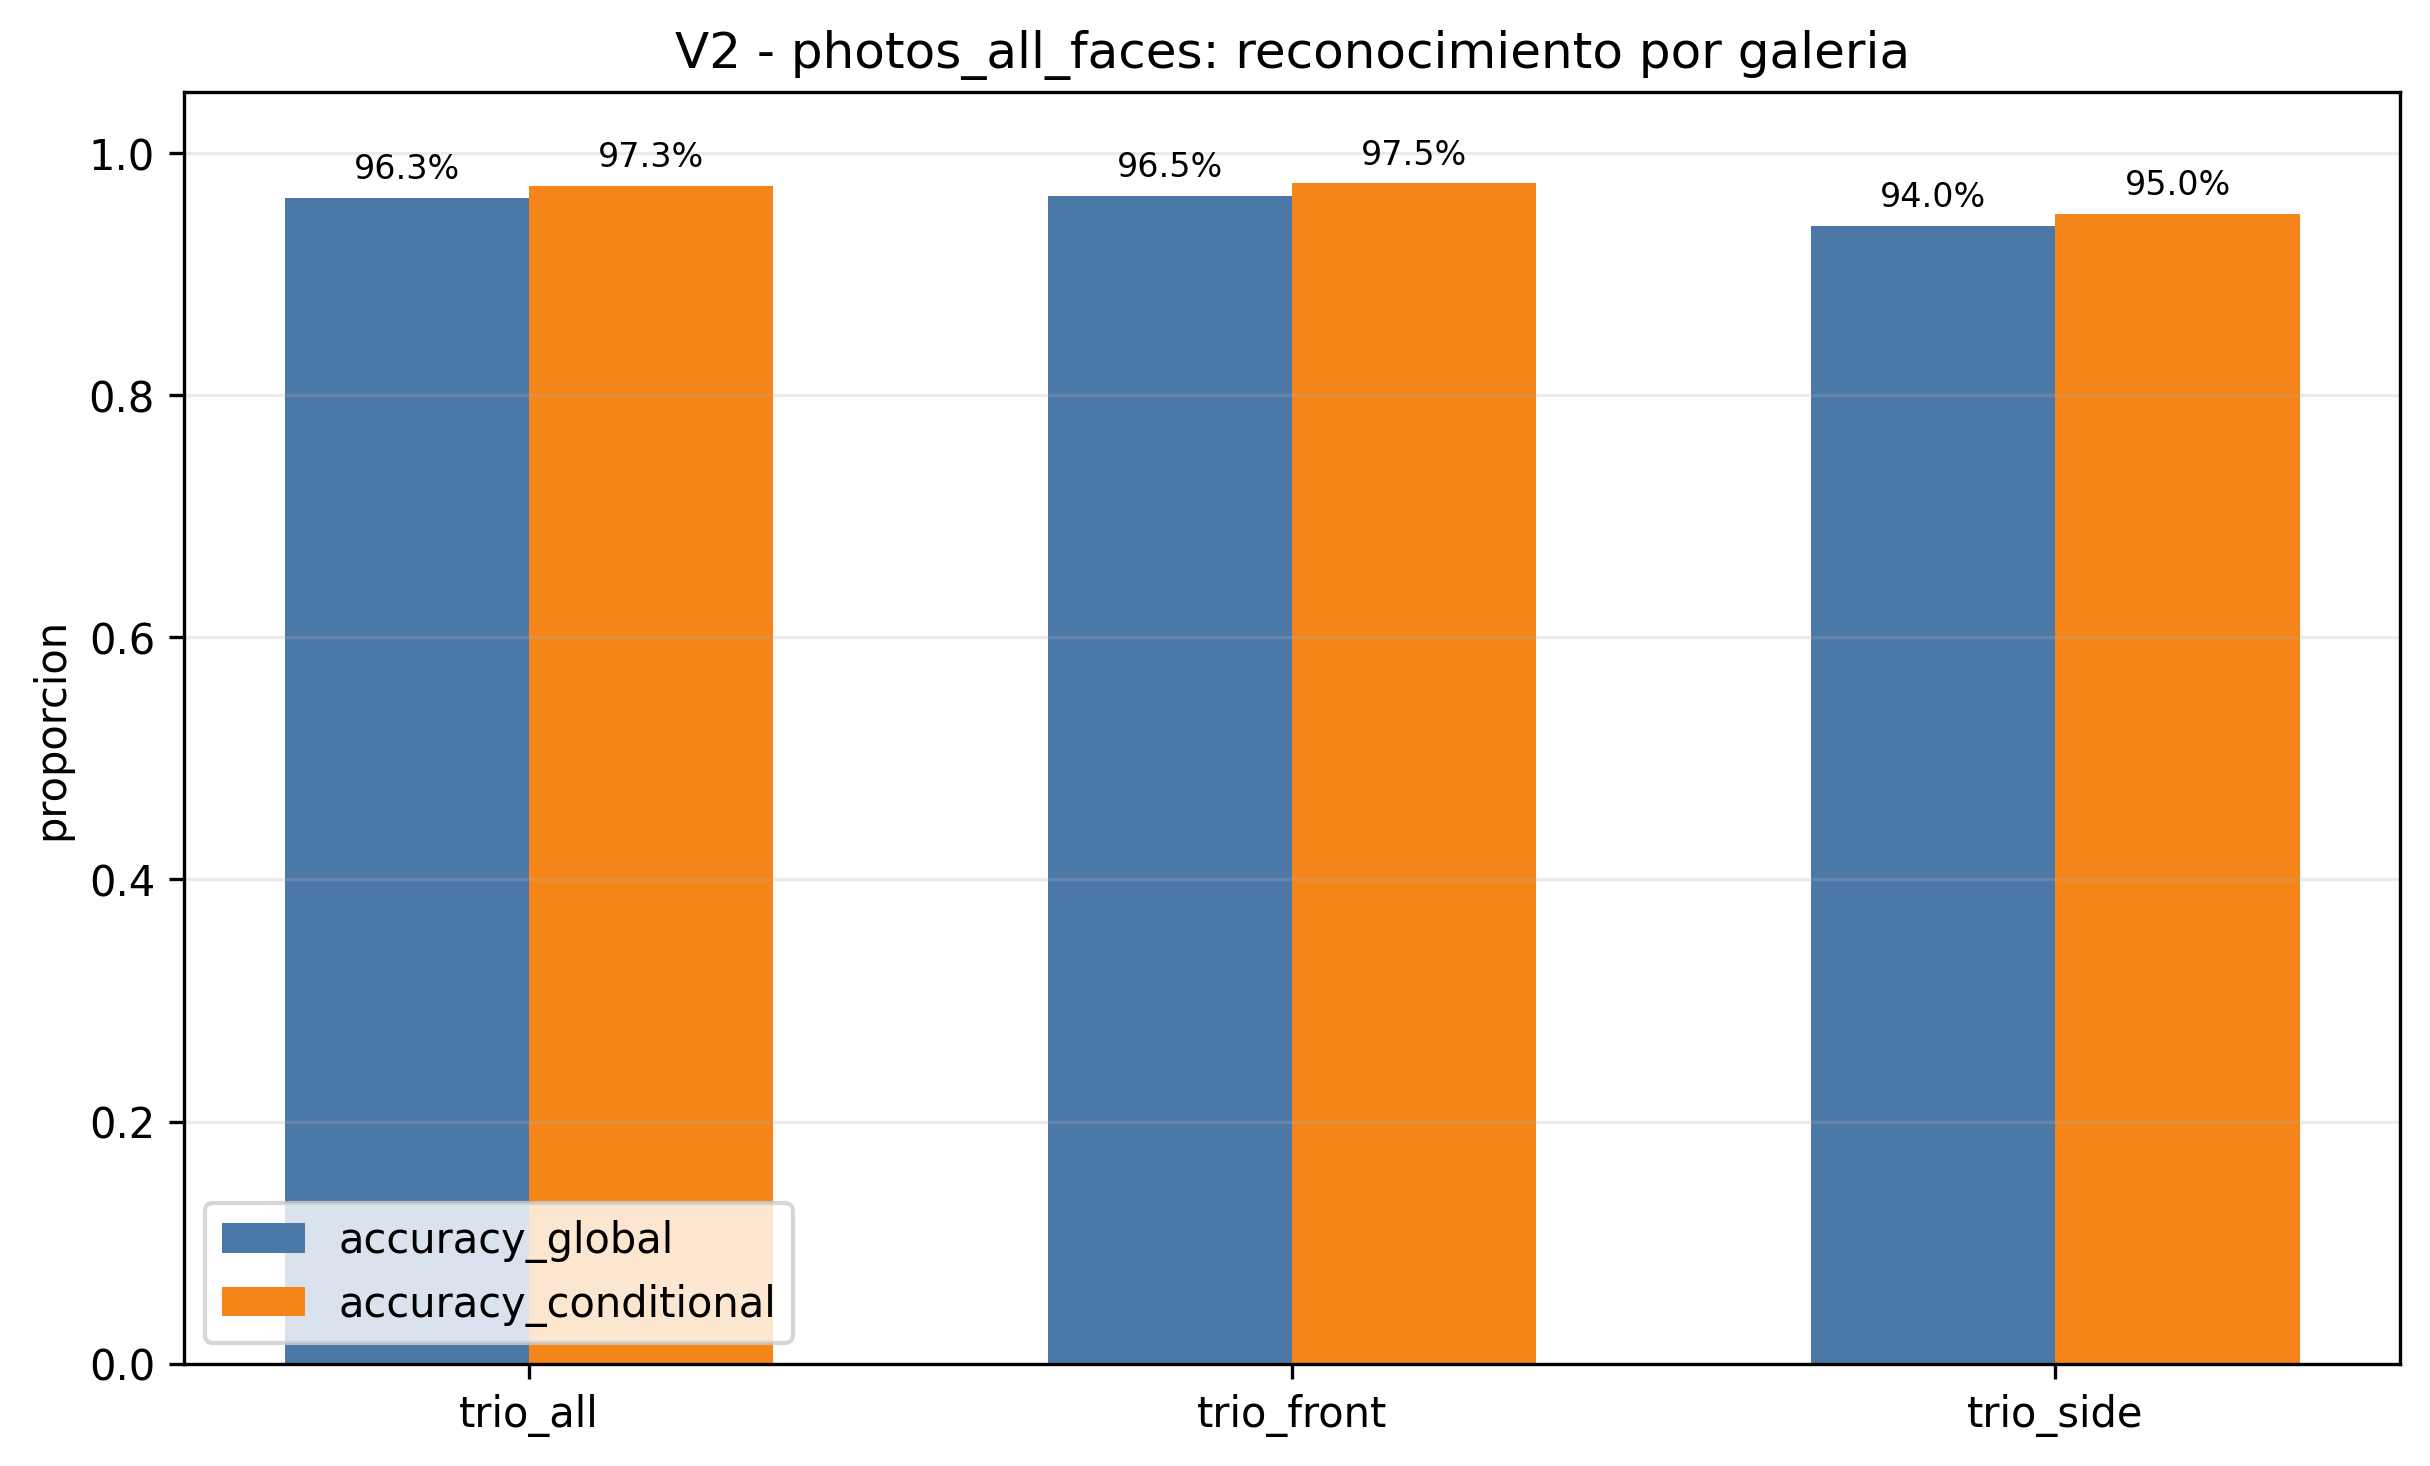
\includegraphics[width=0.88\textwidth]{outputs_v2/figs/metrics/photos_all_faces_pose_comparison.png}
\caption{Comparaci\'on de reconocimiento en \texttt{photos\_all\_faces} para las tres galer\'ias V2. La tasa de detecci\'on es 98.97\% para todas y se reporta en la \autoref{tab:exp_a_galerias}.}
\label{fig:pose_comparison}
\end{figure}

El desglose por sujeto para \texttt{trio\_front} se muestra en la \autoref{tab:exp_a_sujeto}. La identidad \texttt{a} alcanz\'o 100.00\% de acierto global y \texttt{k} obtuvo 99.19\%. Los sujetos con menor desempe\~no fueron \texttt{g} e \texttt{i}, con 93.55\% y 94.35\%, respectivamente. Aun as\'i, todos los sujetos superaron 93\% de \accglobal{}.

\begin{table}[H]
\centering
\caption{Experimento A con \texttt{trio\_front}: resultados por sujeto.}
\label{tab:exp_a_sujeto}
\begin{adjustbox}{max width=\textwidth}
\begin{tabular}{cccccc}
\toprule
Sujeto & Probes & Detectados & Correctos & \texttt{detection\_rate} & \accglobal{} \\
\midrule
\texttt{a} & 124 & 124 & 124 & 100.00\% & 100.00\% \\
\texttt{b} & 124 & 124 & 120 & 100.00\% & 96.77\% \\
\texttt{c} & 124 & 123 & 120 & 99.19\% & 96.77\% \\
\texttt{d} & 124 & 124 & 119 & 100.00\% & 95.97\% \\
\texttt{e} & 124 & 124 & 118 & 100.00\% & 95.16\% \\
\texttt{f} & 124 & 120 & 119 & 96.77\% & 95.97\% \\
\texttt{g} & 124 & 124 & 116 & 100.00\% & 93.55\% \\
\texttt{h} & 124 & 121 & 119 & 97.58\% & 95.97\% \\
\texttt{i} & 124 & 119 & 117 & 95.97\% & 94.35\% \\
\texttt{j} & 124 & 124 & 121 & 100.00\% & 97.58\% \\
\texttt{k} & 124 & 123 & 123 & 99.19\% & 99.19\% \\
\bottomrule
\end{tabular}
\end{adjustbox}
\end{table}

La altura y la distancia afectan el desempe\~no. La \autoref{fig:exp_a_heatmap} resume ambas variables simult\'aneamente: en altura, la peor condici\'on fue 5.0 m, con 92.96\% de \accglobal{}; en distancia, la ca\'ida se vuelve fuerte hacia el final del rango, con 75.00\% a 16.5 m y 79.55\% a 17.0 m.

\begin{figure}[H]
\centering
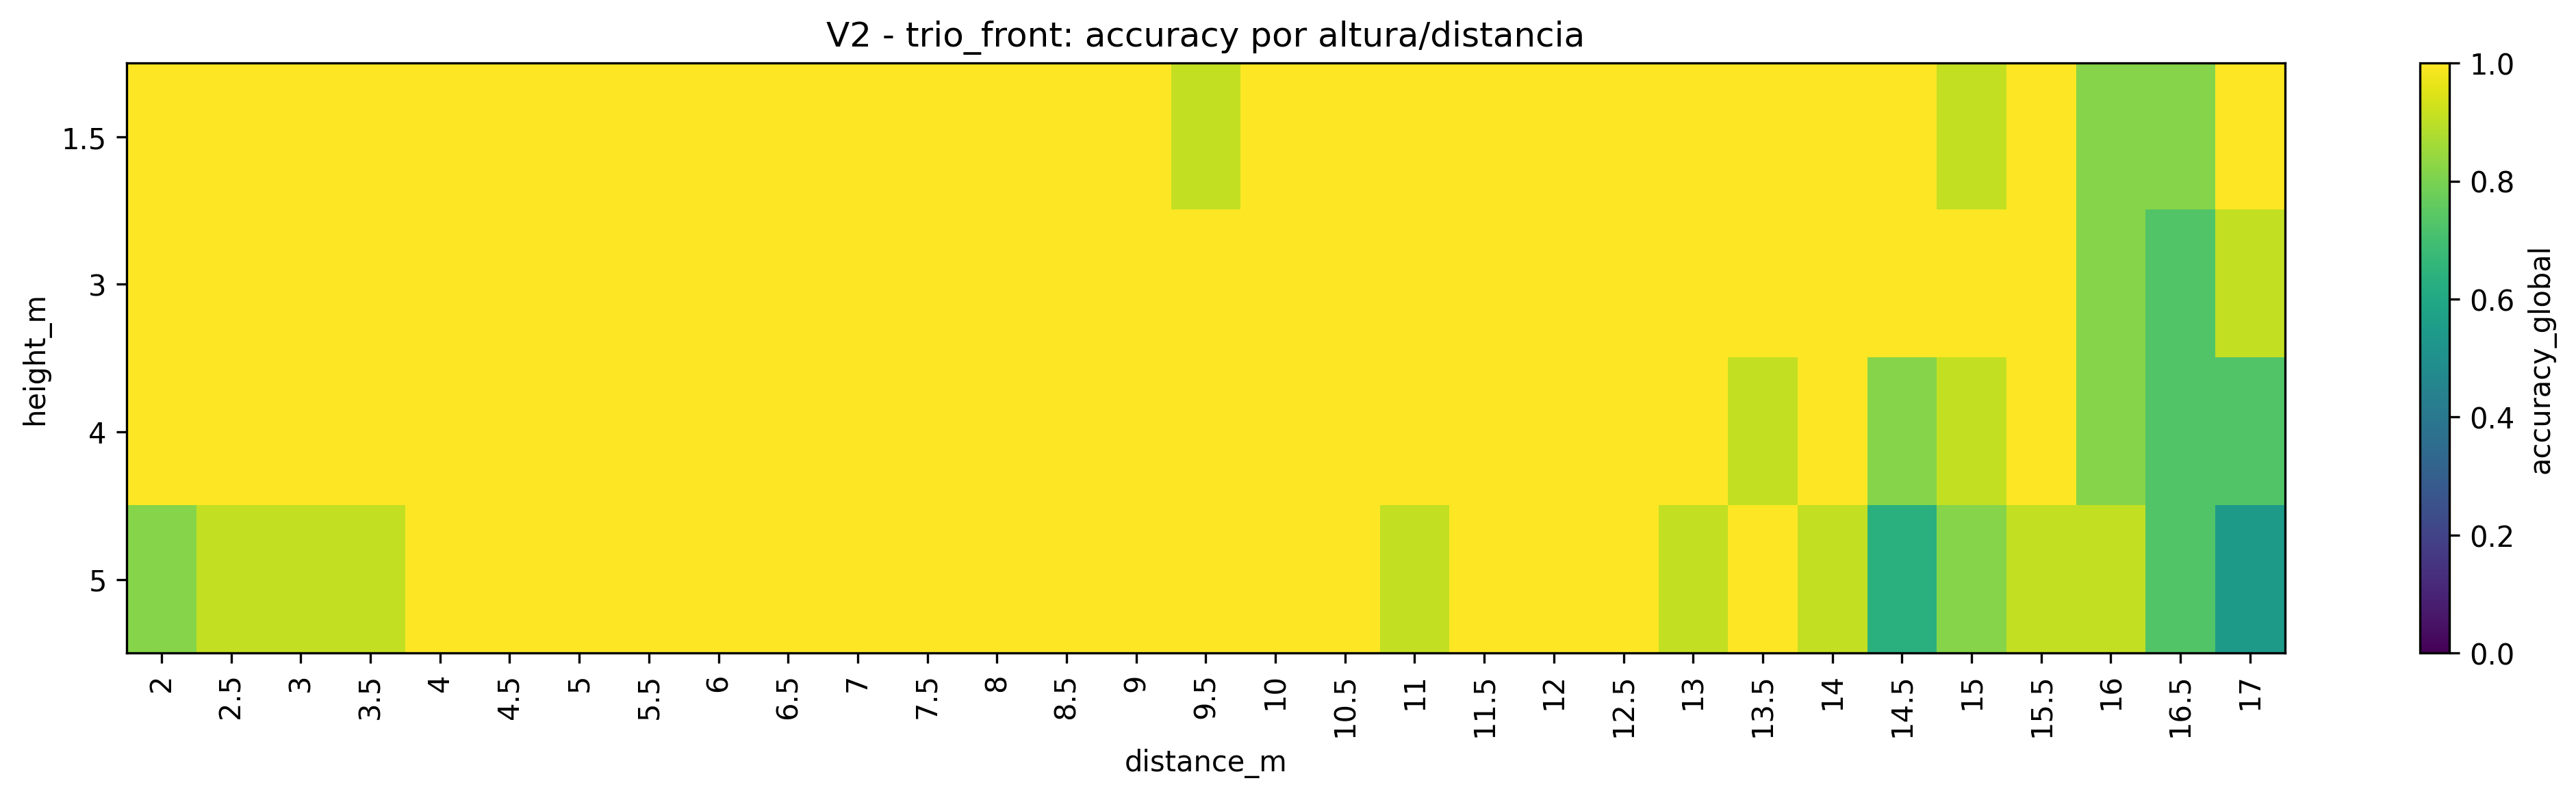
\includegraphics[width=\textwidth]{outputs_v2/figs/metrics/photos_all_faces_trio_front_accuracy_height_distance.png}
\caption{Experimento A con \texttt{trio\_front}: mapa de calor de \accglobal{} por altura y distancia.}
\label{fig:exp_a_heatmap}
\end{figure}

\subsection{Experimento B: im\'agenes completas}

El Experimento B eval\'ua el pipeline completo sobre im\'agenes de dron. La \autoref{tab:exp_b} muestra que la tasa de im\'agenes con al menos una detecci\'on fue 91.45\% para todas las galer\'ias. Con \texttt{trio\_front}, el sistema recuper\'o 1070 identidades de 1364 esperadas.

\begin{table}[H]
\centering
\caption{Experimento B: recuperaci\'on de identidades esperadas en im\'agenes completas.}
\label{tab:exp_b}
\begin{adjustbox}{max width=\textwidth}
\begin{tabular}{lcccccc}
\toprule
Galer\'ia & Im\'agenes & Im\'agenes con detecci\'on & Esperadas & Recuperadas & Inesperadas & Recall global \\
\midrule
\texttt{trio\_front} & 620 & 567 & 1364 & 1070 & 42 & 78.45\% \\
\texttt{trio\_side} & 620 & 567 & 1364 & 1050 & 65 & 76.98\% \\
\texttt{trio\_all} & 620 & 567 & 1364 & 1064 & 50 & 78.01\% \\
\bottomrule
\end{tabular}
\end{adjustbox}
\end{table}

Para \texttt{trio\_front}, el desglose de la \autoref{tab:exp_b_set} indica que el sistema recuper\'o al menos una identidad esperada en 559 de 620 im\'agenes (90.16\%), recuper\'o todas las identidades esperadas en 420 im\'agenes (67.74\%) y obtuvo coincidencia exacta del conjunto esperado en 399 im\'agenes (64.35\%). La similitud de Jaccard media fue 77.22\%.

\begin{table}[H]
\centering
\caption{M\'etricas de conjunto para \texttt{trio\_front} en el Experimento B.}
\label{tab:exp_b_set}
\begin{tabular}{lc}
\toprule
M\'etrica & Valor \\
\midrule
\texttt{image\_detection\_rate} & 91.45\% \\
\texttt{expected\_identity\_recall\_global} & 78.45\% \\
\texttt{any\_expected\_found\_rate} & 90.16\% \\
\texttt{all\_expected\_found\_rate} & 67.74\% \\
\texttt{exact\_expected\_set\_match\_rate} & 64.35\% \\
\texttt{mean\_jaccard\_set\_similarity} & 77.22\% \\
\bottomrule
\end{tabular}
\end{table}

La \autoref{fig:full_image_examples} ilustra el tipo de salida que produce el pipeline sobre im\'agenes completas. Se muestran recortes de contexto y zooms de las cajas detectadas para que las caras sean visibles en el PDF.

\begin{figure}[H]
\centering
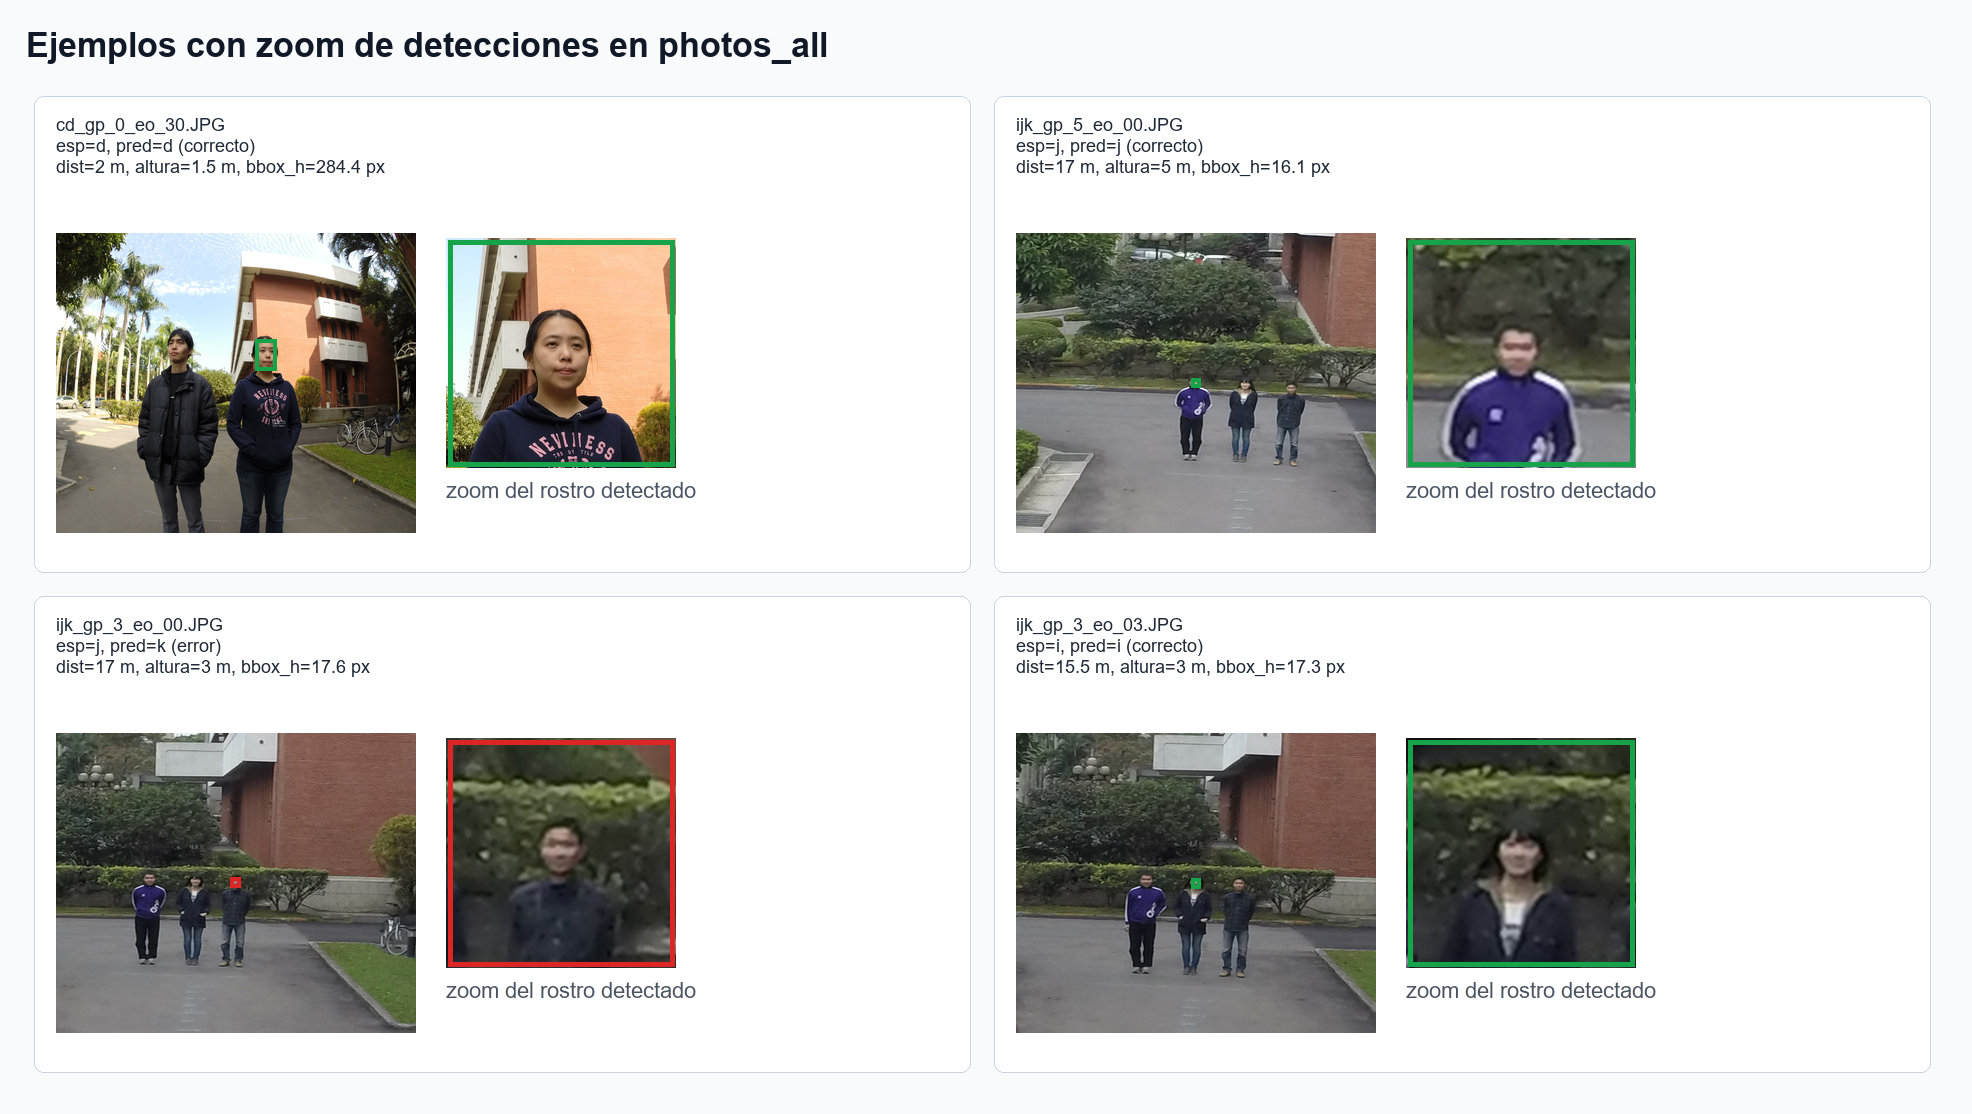
\includegraphics[width=\textwidth]{figs/detection/droneface_full_image_detection_zooms.png}
\caption{Ejemplos ampliados del flujo sobre im\'agenes completas: contexto de la detecci\'on, zoom del rostro e identidad predicha.}
\label{fig:full_image_examples}
\end{figure}

El mapa de la \autoref{fig:exp_b_recall} muestra que el pipeline completo es mucho m\'as sensible a la escala del rostro que el Experimento A. Con \texttt{trio\_front}, el recall global se mantiene alto hasta cerca de 10 m, pero cae a 40.91\% en 13.5 m, 27.27\% en 15.0 m y 15.91\% en 17.0 m. Esta tendencia sugiere que la dificultad principal de las im\'agenes completas est\'a en detectar y representar rostros peque\~nos, no solo en comparar embeddings.

\begin{figure}[H]
\centering
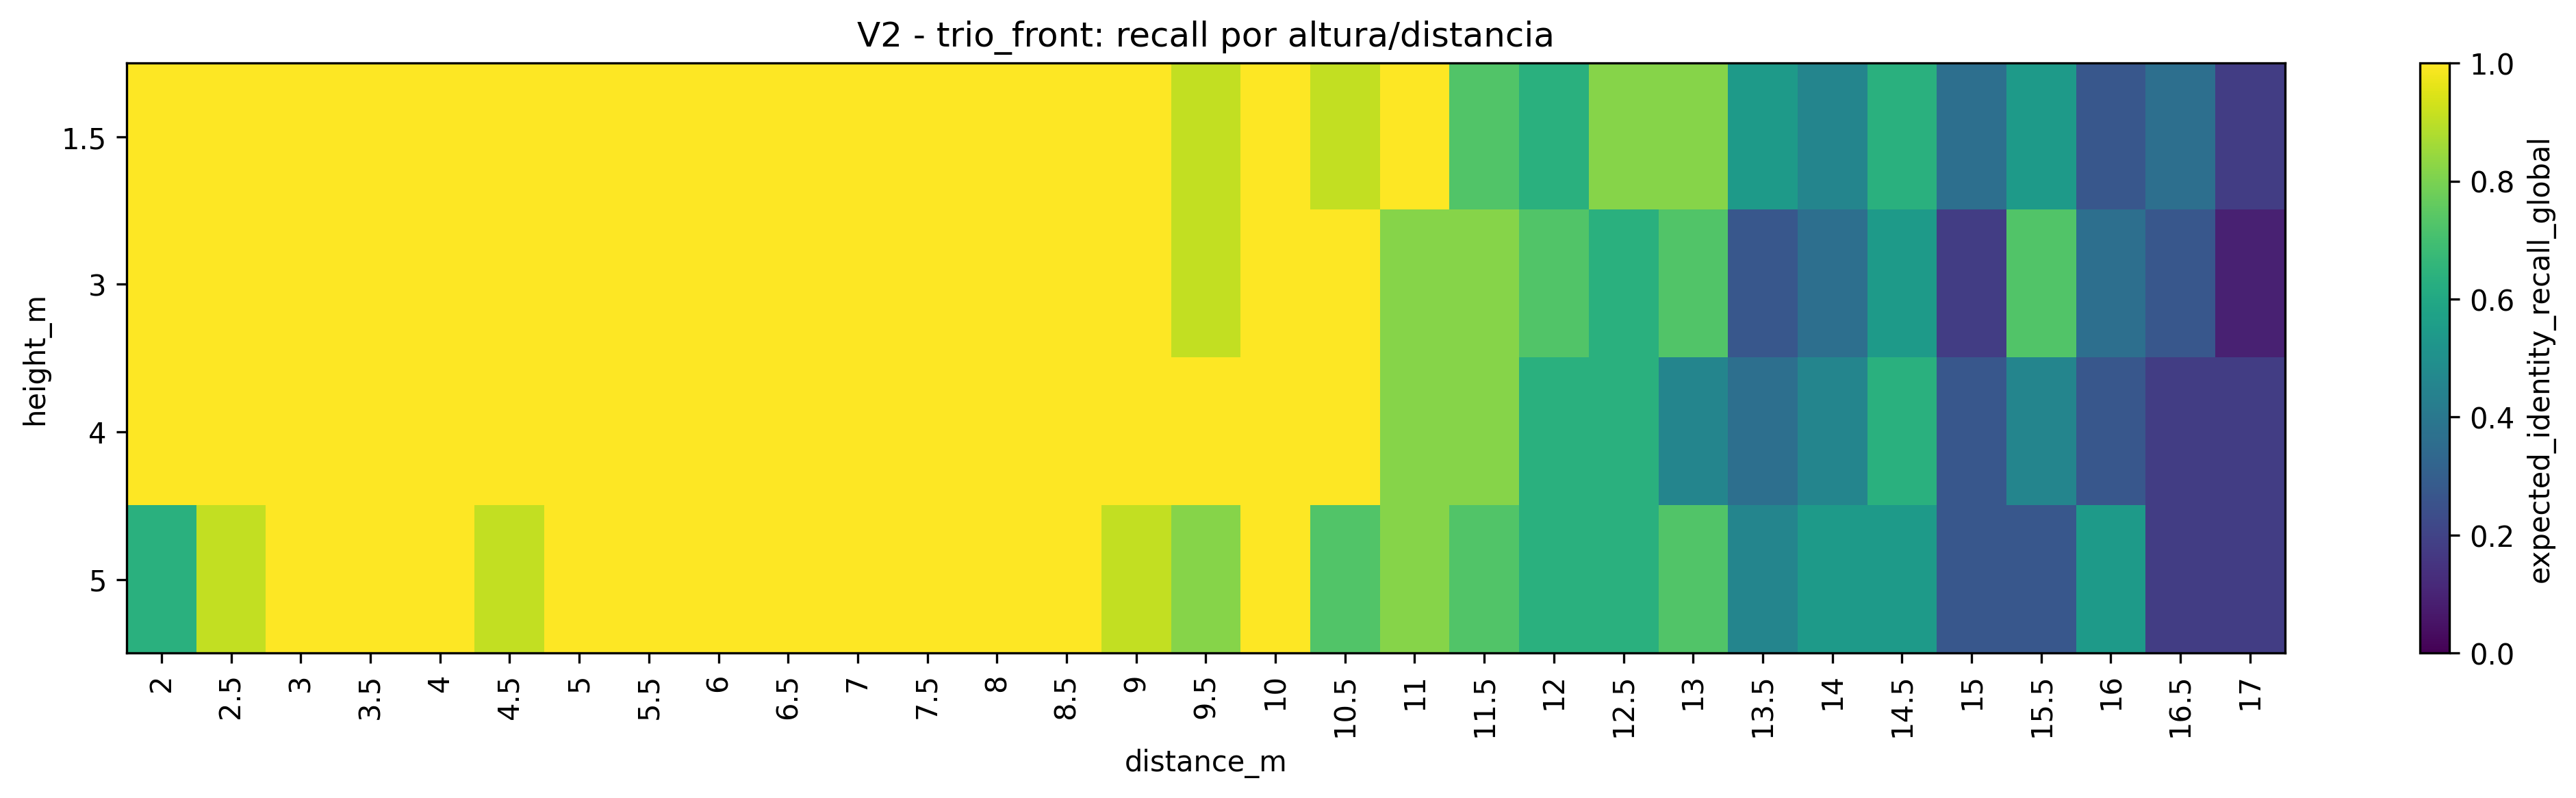
\includegraphics[width=\textwidth]{outputs_v2/figs/metrics/photos_all_trio_front_recall_height_distance.png}
\caption{Experimento B con \texttt{trio\_front}: recuperaci\'on de identidades esperadas por altura y distancia.}
\label{fig:exp_b_recall}
\end{figure}

\subsection{Experimento C: bbox-level}

El Experimento C entrega una evaluaci\'on m\'as estricta porque compara cada posici\'on espacial esperada con la caja detectada correspondiente. La \autoref{tab:exp_c_galerias} muestra que \texttt{trio\_front} obtuvo F1 global de 79.77\%, con 88.33\% de precisi\'on y 72.73\% de recall. La diferencia entre precisi\'on y recall indica que el sistema suele ser relativamente confiable cuando asigna una identidad, pero a\'un pierde un n\'umero relevante de sujetos esperados.

\begin{table}[H]
\centering
\caption{Experimento C: m\'etricas \textit{bbox-level} por galer\'ia.}
\label{tab:exp_c_galerias}
\begin{adjustbox}{max width=\textwidth}
\begin{tabular}{lccccccc}
\toprule
Galer\'ia & Slots & TP & FP & FN & Precisi\'on & Recall & F1 \\
\midrule
\texttt{trio\_front} & 1394 & 992 & 131 & 372 & 88.33\% & 72.73\% & 79.77\% \\
\texttt{trio\_side} & 1394 & 970 & 153 & 394 & 86.38\% & 71.11\% & 78.01\% \\
\texttt{trio\_all} & 1394 & 985 & 138 & 379 & 87.71\% & 72.21\% & 79.21\% \\
\bottomrule
\end{tabular}
\end{adjustbox}
\end{table}

La \autoref{fig:bbox_gallery} muestra esta comparaci\'on entre galer\'ias: \texttt{trio\_front} queda levemente sobre \texttt{trio\_all} y \texttt{trio\_side}.

\begin{figure}[H]
\centering
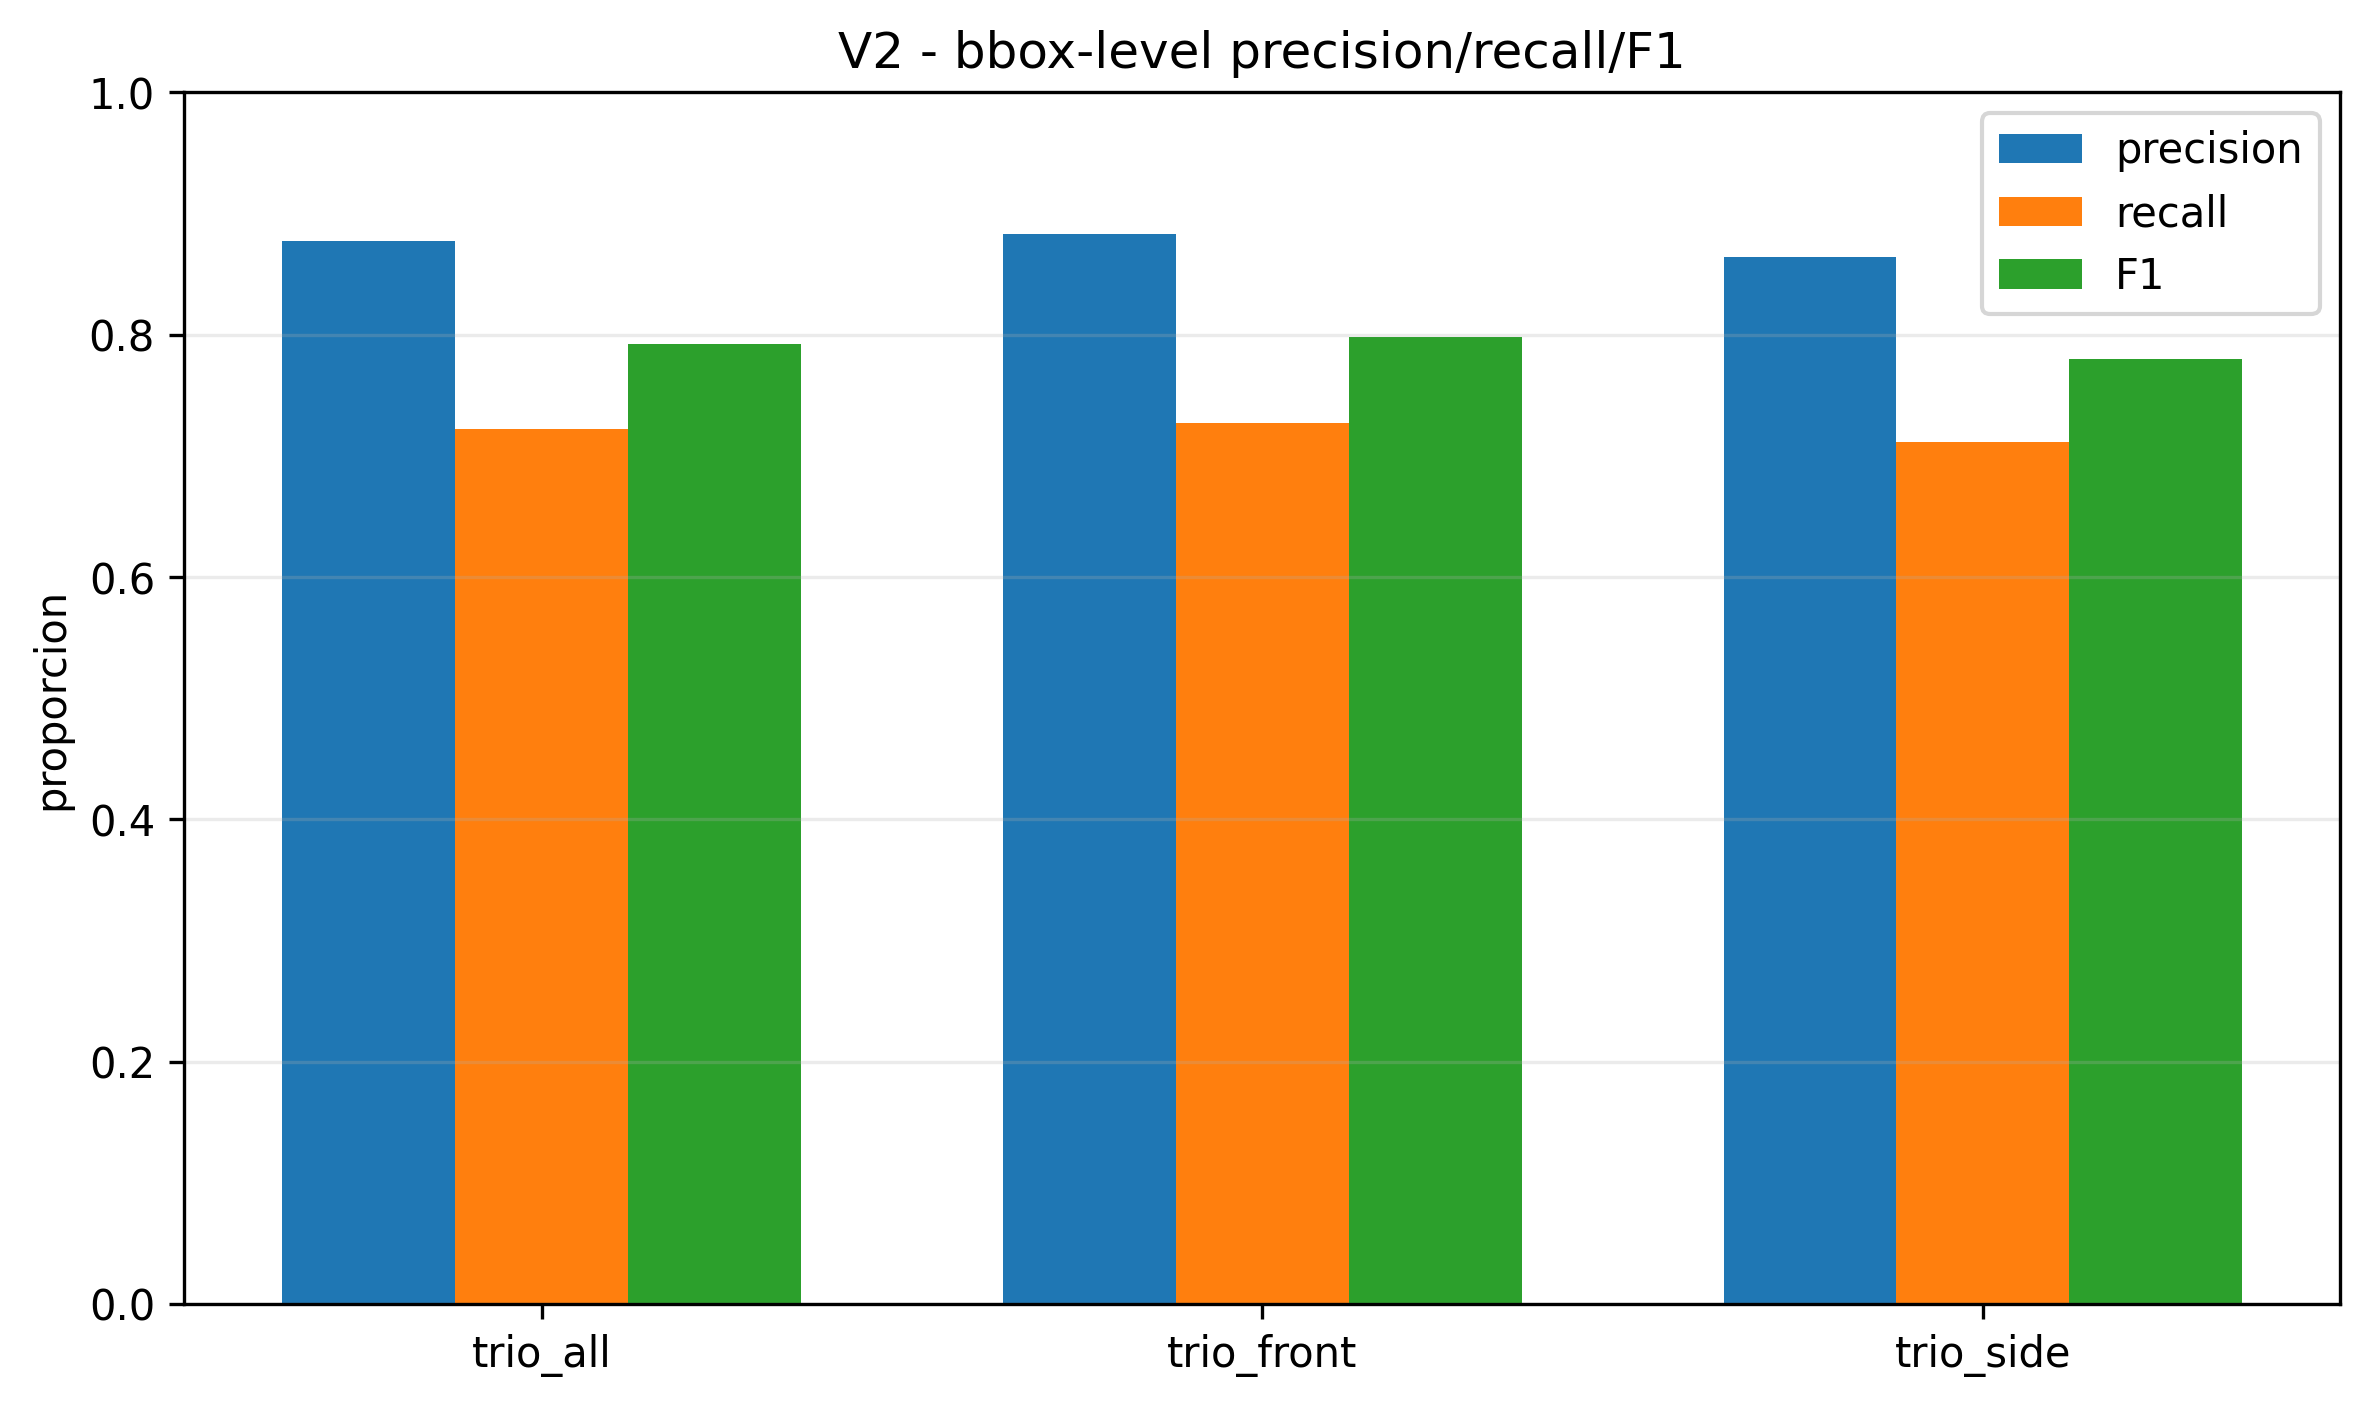
\includegraphics[width=0.88\textwidth]{outputs_v2/figs/metrics/photos_all_bbox_precision_recall_f1_by_gallery.png}
\caption{Experimento C: precisi\'on, recall y F1 por galer\'ia.}
\label{fig:bbox_gallery}
\end{figure}

El an\'alisis por prefijo de la \autoref{tab:bbox_prefix} muestra que \texttt{ab} y \texttt{gh} fueron los casos m\'as favorables para \texttt{trio\_front}, con F1 de 84.60\% y 81.92\%, respectivamente. El prefijo \texttt{ijk}, que contiene tres personas, obtuvo 76.36\%, lo que sugiere que las im\'agenes con m\'as sujetos aumentan la probabilidad de omisiones o asignaciones incorrectas.

\begin{table}[H]
\centering
\caption{Experimento C con \texttt{trio\_front}: m\'etricas por prefijo de imagen.}
\label{tab:bbox_prefix}
\begin{adjustbox}{max width=\textwidth}
\begin{tabular}{lccccccc}
\toprule
Prefijo & Slots & TP & FP & FN & Precisi\'on & Recall & F1 \\
\midrule
\texttt{ab} & 249 & 195 & 18 & 53 & 91.55\% & 78.63\% & 84.60\% \\
\texttt{cd} & 264 & 194 & 45 & 54 & 81.17\% & 78.23\% & 79.67\% \\
\texttt{ef} & 256 & 172 & 22 & 76 & 88.66\% & 69.35\% & 77.83\% \\
\texttt{gh} & 251 & 179 & 10 & 69 & 94.71\% & 72.18\% & 81.92\% \\
\texttt{ijk} & 374 & 252 & 36 & 120 & 87.50\% & 67.74\% & 76.36\% \\
\bottomrule
\end{tabular}
\end{adjustbox}
\end{table}

La \autoref{fig:bbox_prefix} resume la variaci\'on por composici\'on del grupo. En cambio, la \autoref{fig:bbox_distance} muestra la ca\'ida por distancia con una curva por galer\'ia, lo que hace m\'as visible el quiebre de desempe\~no en el tramo final. Las oscilaciones sobre 13 m deben interpretarse con cautela: cada punto corresponde a un subconjunto de la evaluaci\'on, por lo que pocos cambios absolutos en TP, FP o FN producen variaciones visibles en F1.

\begin{figure}[H]
\centering
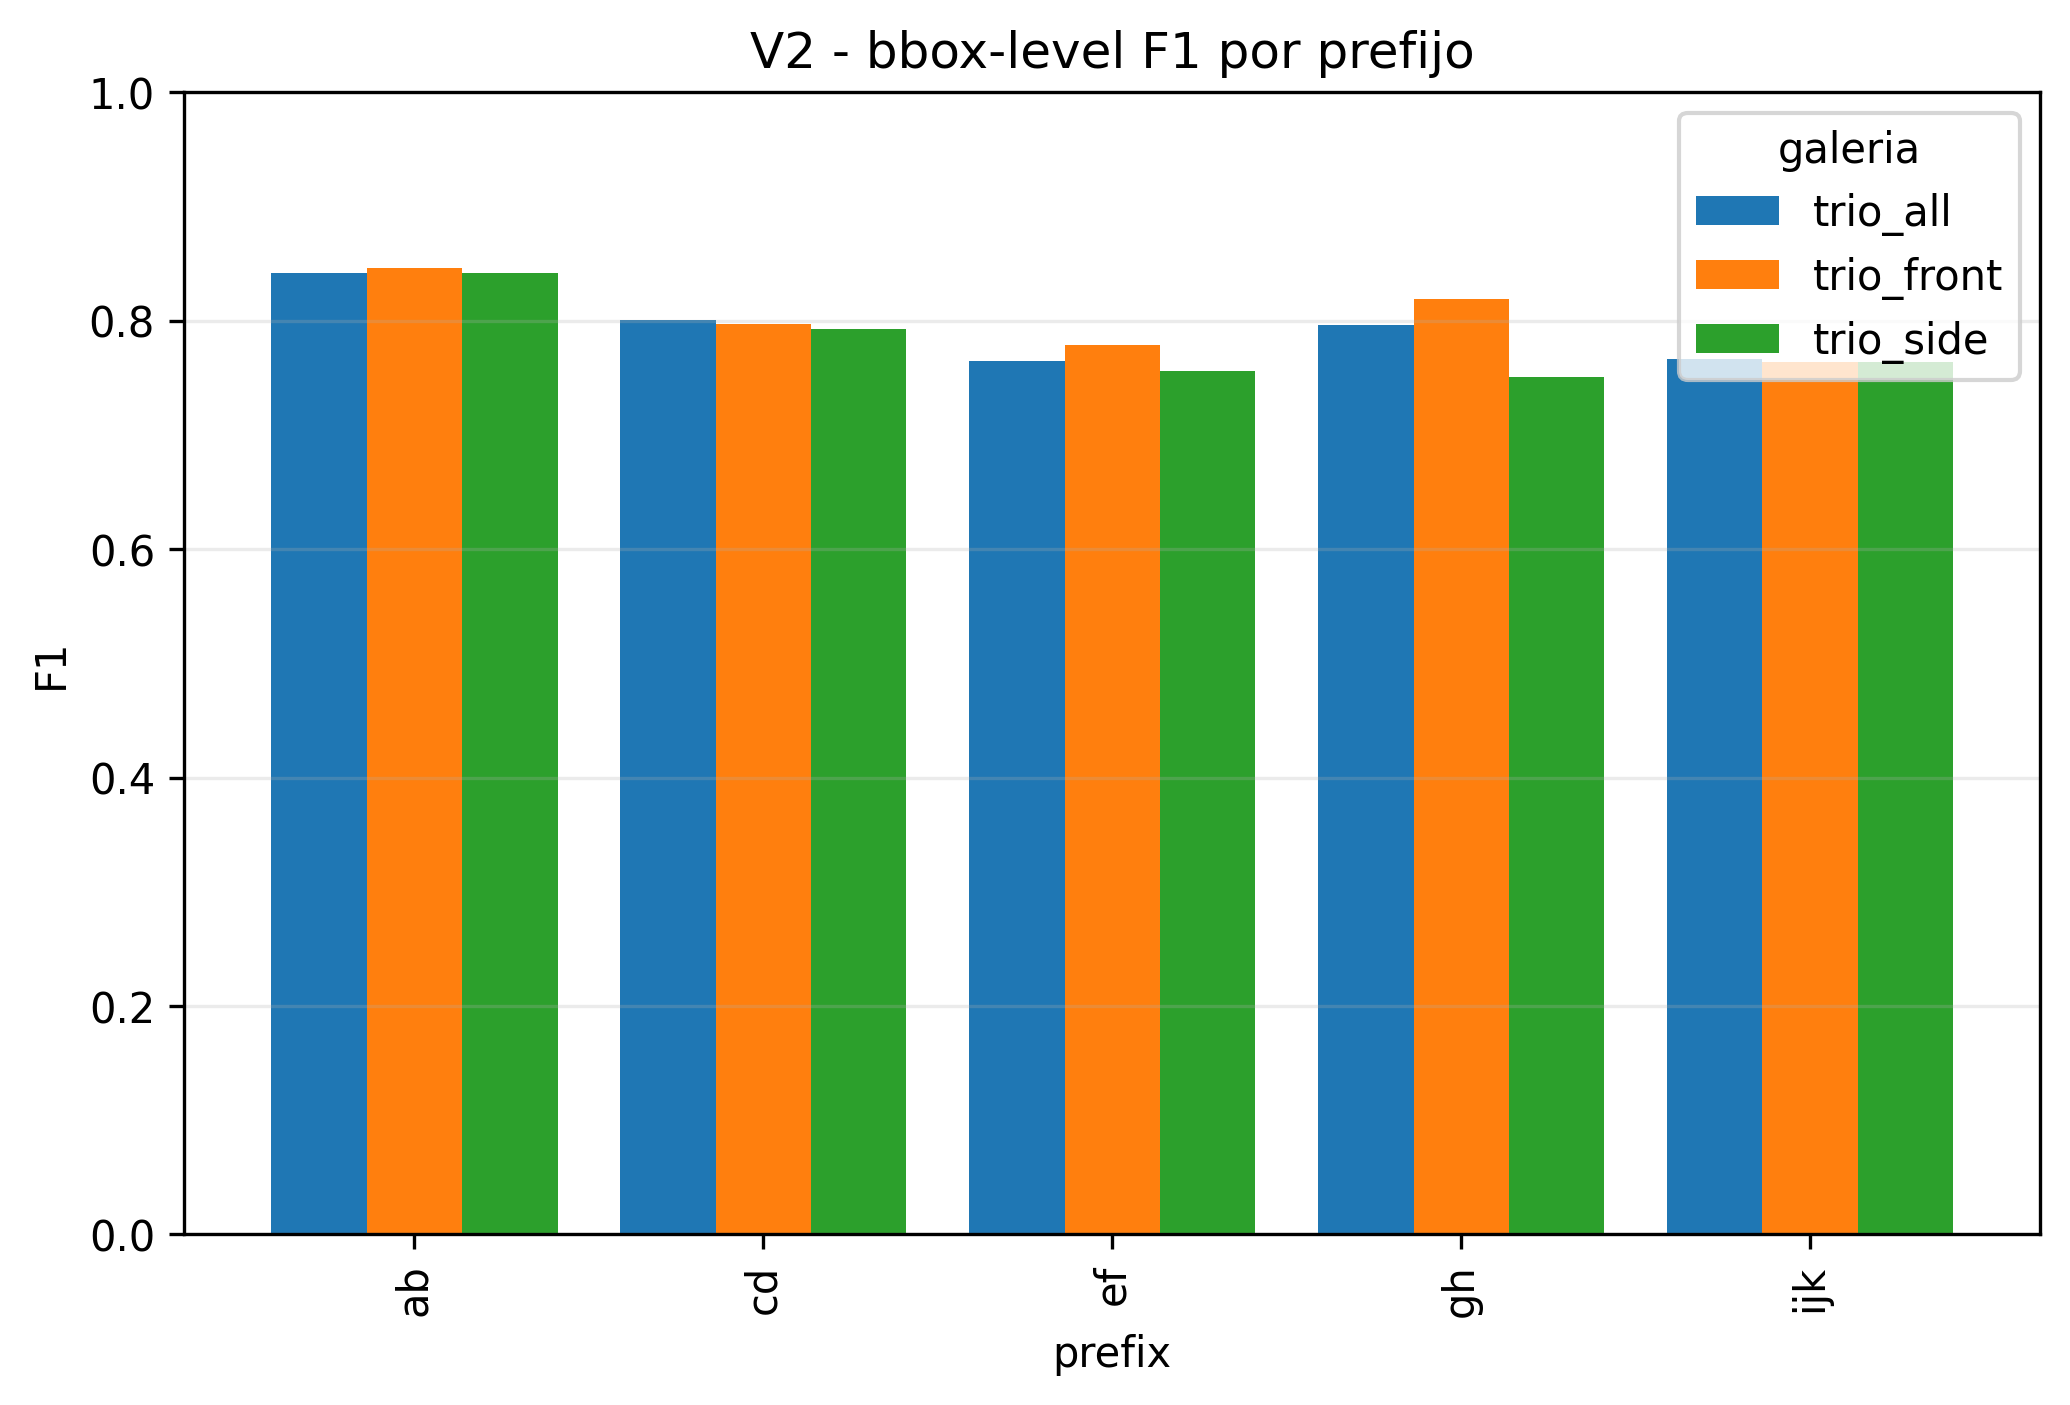
\includegraphics[width=0.86\textwidth]{outputs_v2/figs/metrics/photos_all_bbox_f1_by_prefix.png}
\caption{Experimento C: F1 \textit{bbox-level} por prefijo de imagen.}
\label{fig:bbox_prefix}
\end{figure}

\begin{figure}[H]
\centering
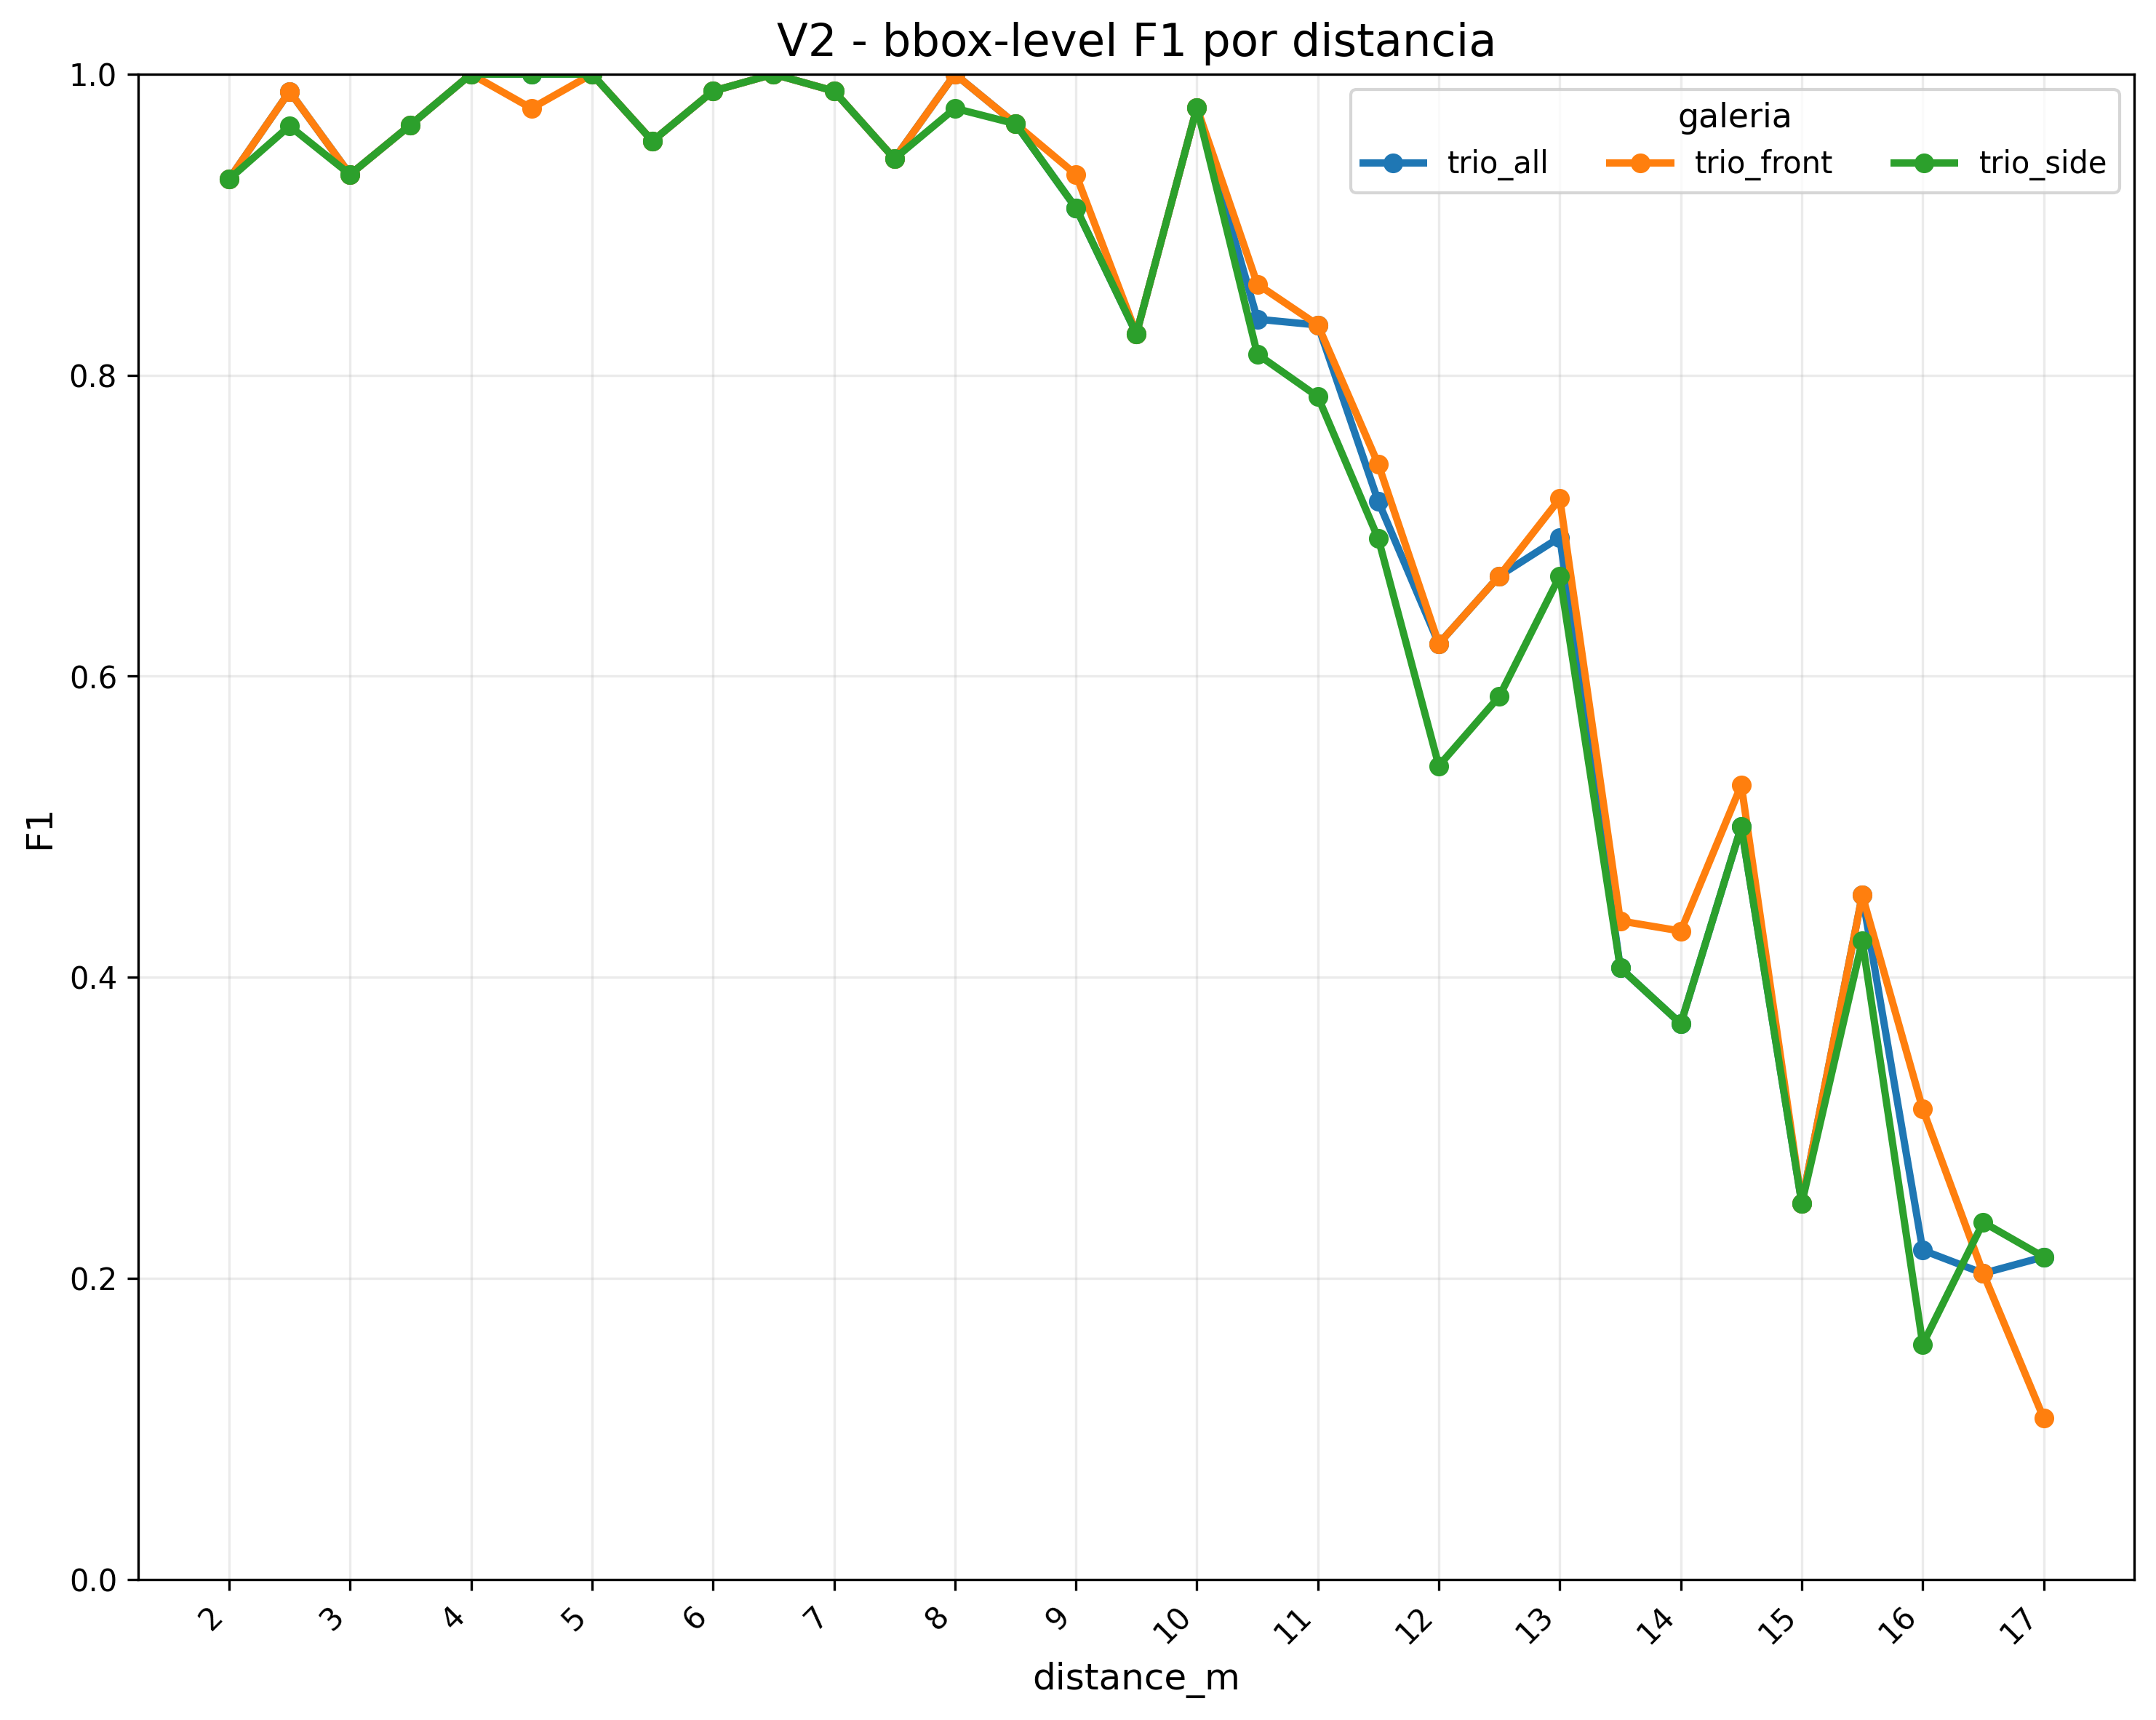
\includegraphics[width=\textwidth]{outputs_v2/figs/metrics/photos_all_bbox_f1_by_distance.png}
\caption{Experimento C: F1 \textit{bbox-level} por distancia, con una curva por galer\'ia.}
\label{fig:bbox_distance}
\end{figure}

\subsection{Verification/AUC y umbral de desconocido}

La \autoref{tab:verification_auc} resume el protocolo de verificaci\'on con \texttt{trio\_front}. El resultado m\'as importante para comparar con sistemas completos es \texttt{photos\_all\_bbox} en modo end-to-end, porque incluye detecci\'on y reconocimiento sobre im\'agenes completas. Ese protocolo obtuvo AUC de 0.822. En cambio, el modo \textit{detected-only} obtuvo AUC de 0.953, lo que indica que el reconocimiento es fuerte cuando la etapa de detecci\'on ya encontr\'o una cara. La evaluaci\'on sobre \texttt{photos\_all\_faces} alcanza AUC de 0.978, pero debe interpretarse como una condici\'on optimista porque parte de rostros ya recortados.

\begin{table}[H]
\centering
\caption{AUC del protocolo de verificaci\'on con \texttt{trio\_front}.}
\label{tab:verification_auc}
\begin{adjustbox}{max width=\textwidth}
\begin{tabular}{llcccc}
\toprule
Conjunto & Lectura & Pares & Matches & Mismatches & AUC \\
\midrule
\texttt{photos\_all\_faces} & Global & 15004 & 1364 & 13640 & 0.978 \\
\texttt{photos\_all\_faces} & Detected-only & 14850 & 1350 & 13500 & 0.986 \\
\texttt{photos\_all\_bbox} & End-to-end & 15334 & 1364 & 13970 & 0.822 \\
\texttt{photos\_all\_bbox} & Detected-only & 12353 & 1093 & 11260 & 0.953 \\
\bottomrule
\end{tabular}
\end{adjustbox}
\end{table}

La \autoref{fig:roc_bbox} muestra por qu\'e es \'util reportar ambas curvas. La ROC end-to-end incluye las caras no detectadas como pares con puntaje cero, por lo que aparece un salto cuando el umbral cruza ese valor. La ROC \textit{detected-only} elimina esas filas y permite observar la calidad del reconocimiento condicionado a detecci\'on.

\begin{figure}[H]
\centering
\begin{subfigure}{0.48\textwidth}
    \centering
    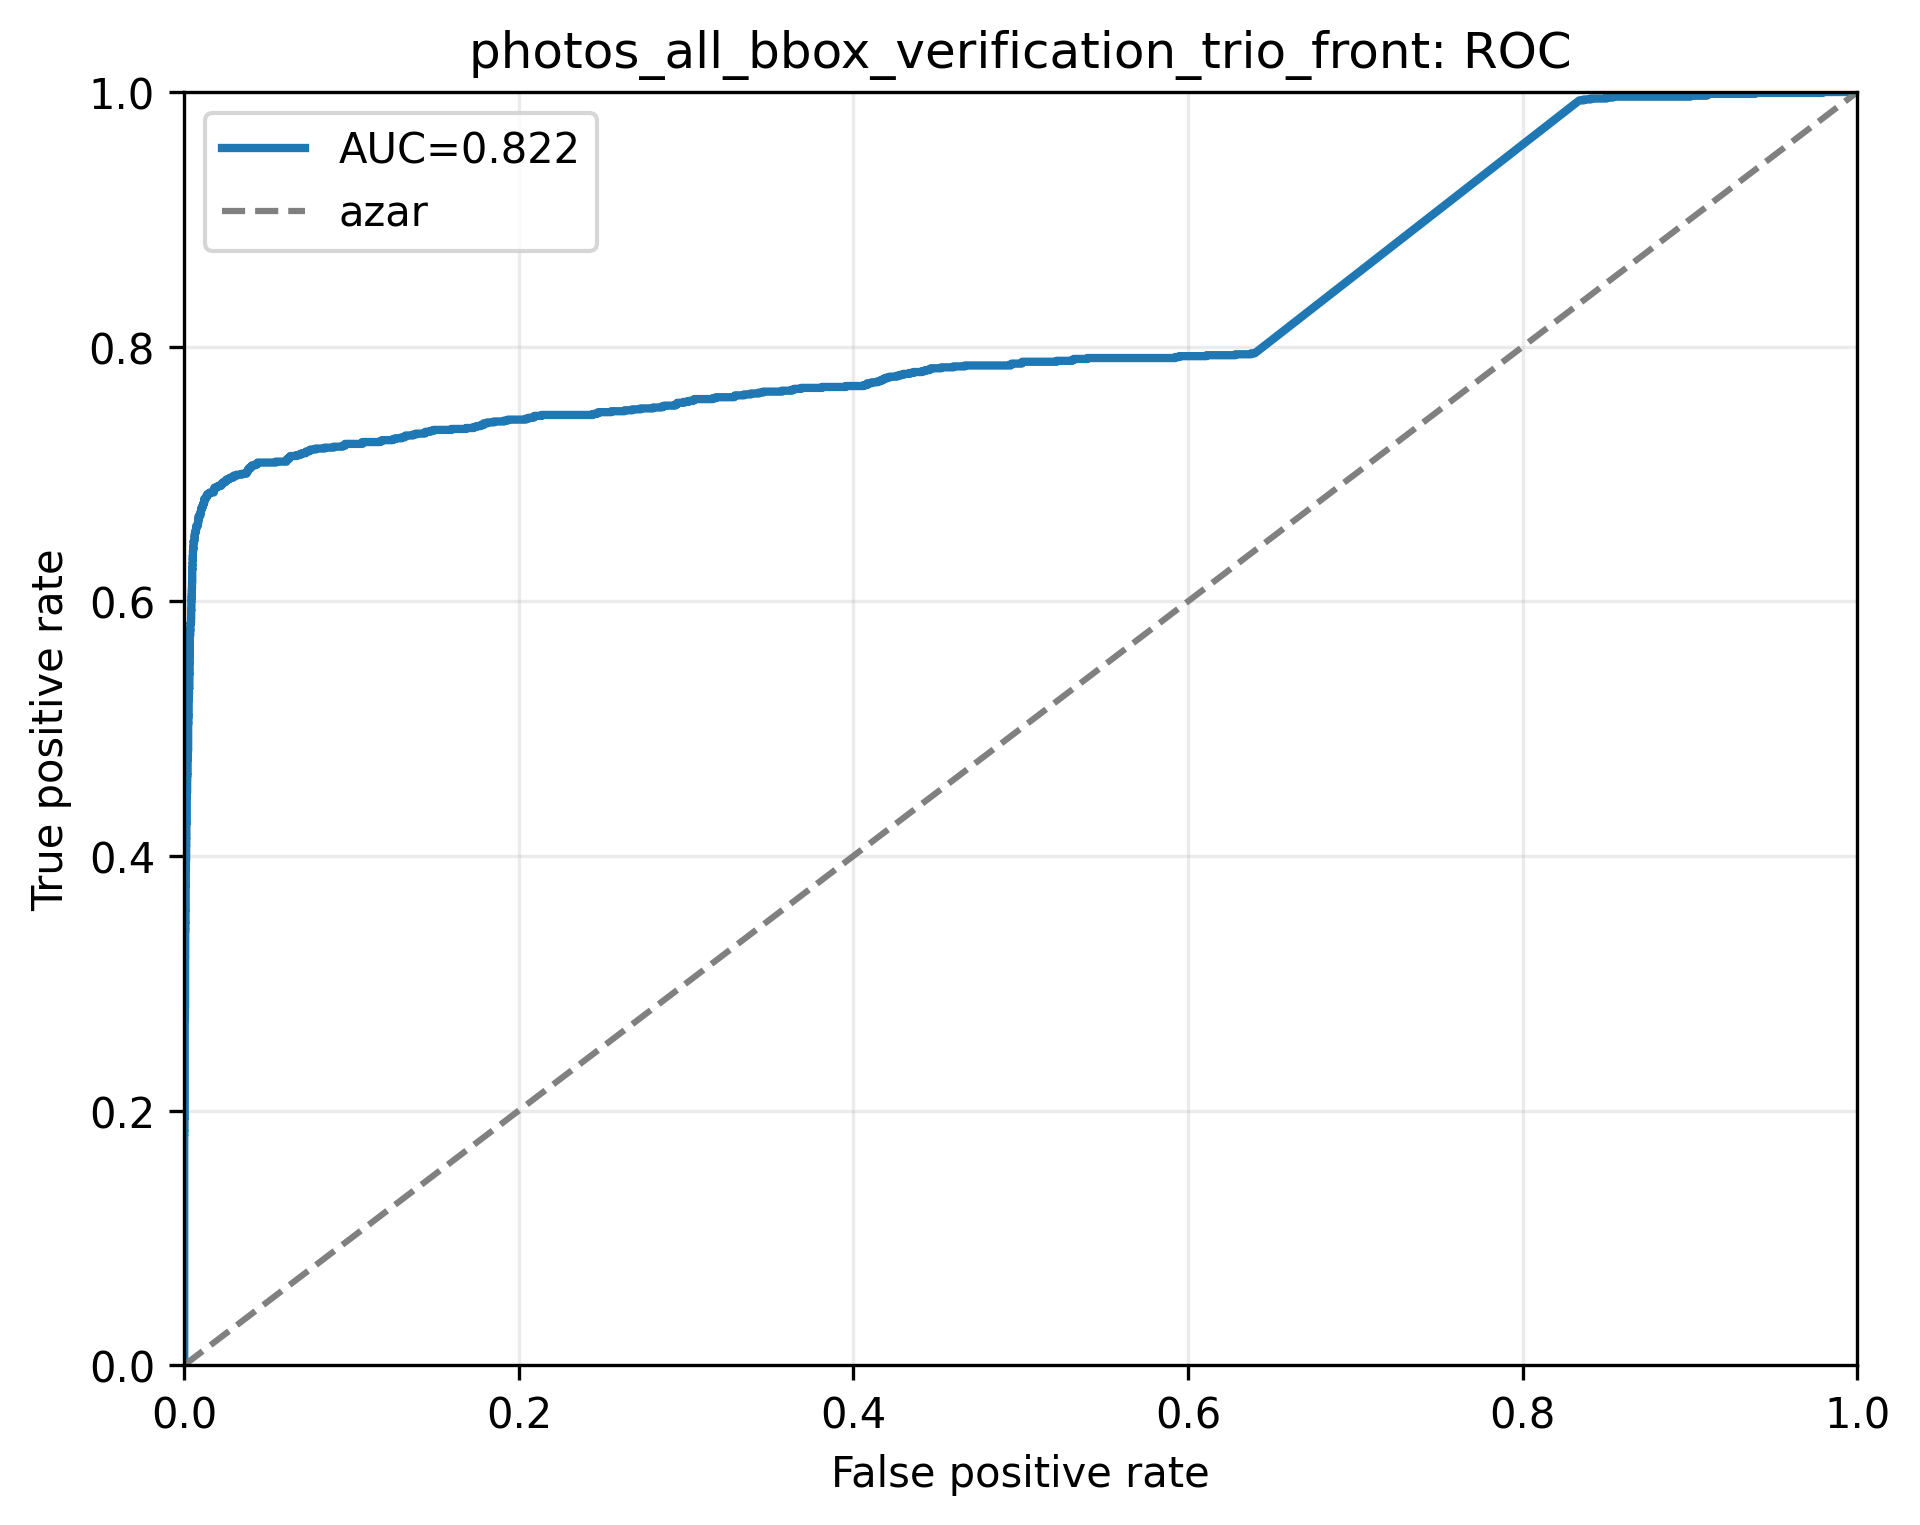
\includegraphics[width=\textwidth]{outputs_v2/figs/metrics/photos_all_bbox_verification_trio_front_roc.png}
    \caption{End-to-end.}
\end{subfigure}
\hfill
\begin{subfigure}{0.48\textwidth}
    \centering
    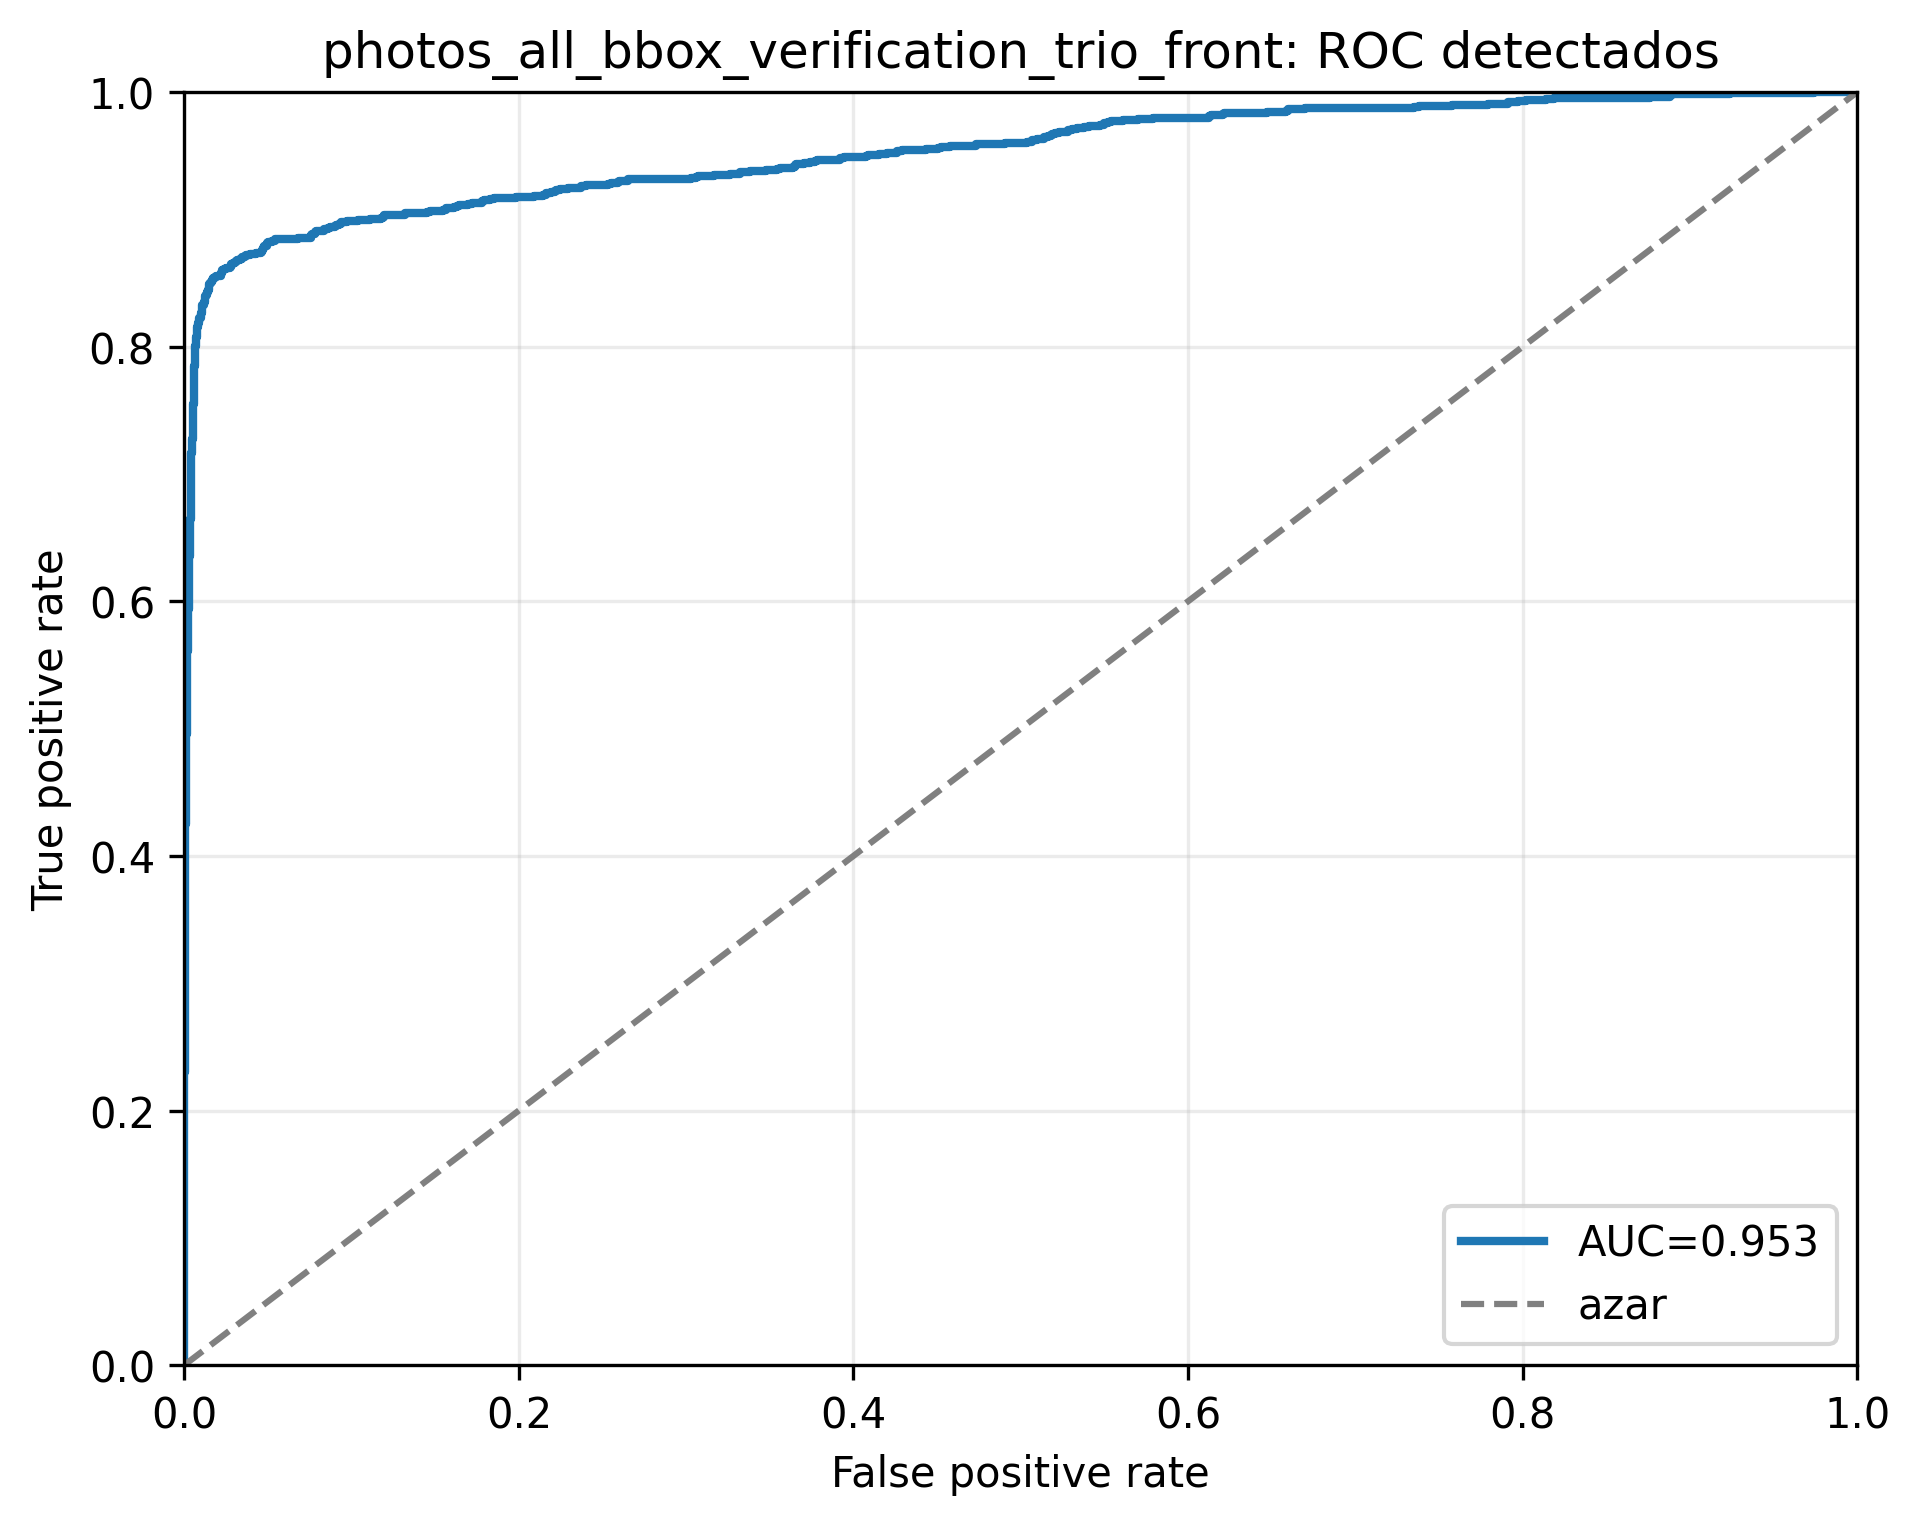
\includegraphics[width=\textwidth]{outputs_v2/figs/metrics/photos_all_bbox_verification_trio_front_roc_detected_only.png}
    \caption{Detected-only.}
\end{subfigure}
\caption{Curvas ROC para \texttt{photos\_all\_bbox} con \texttt{trio\_front}.}
\label{fig:roc_bbox}
\end{figure}

La separaci\'on entre detecci\'on y reconocimiento se resume en la \autoref{tab:detection_recognition_split}. De 1364 caras esperadas, 1093 fueron asociadas a una detecci\'on, lo que equivale a 80.13\% de recall del detector por slot esperado. Entre esas caras detectadas, 992 fueron reconocidas correctamente, es decir, 90.76\% de exactitud condicionada a detecci\'on. Esta lectura explica la diferencia entre el AUC end-to-end y el AUC \textit{detected-only} de la \autoref{tab:verification_auc}.

\begin{table}[H]
\centering
\caption{Separaci\'on entre detecci\'on y reconocimiento en \texttt{photos\_all} con \texttt{trio\_front}.}
\label{tab:detection_recognition_split}
\begin{adjustbox}{max width=\textwidth}
\begin{tabular}{lc}
\toprule
Cantidad o m\'etrica & Valor \\
\midrule
Caras esperadas & 1364 \\
Caras esperadas con detecci\'on asociada & 1093 \\
Caras esperadas sin detecci\'on & 271 \\
Detecciones extra & 30 \\
Recall del detector por slot esperado & 80.13\% \\
Reconocimiento correcto condicionado a detecci\'on & 90.76\% \\
\bottomrule
\end{tabular}
\end{adjustbox}
\end{table}

\subsection{Tama\~no de rostro detectado y confiabilidad}
\label{sec:bbox_size}

Para explicar la ca\'ida observada a distancias largas, se agreg\'o un an\'alisis liviano usando las cajas ya guardadas por el pipeline. La \autoref{tab:bbox_size_metrics} agrupa las detecciones esperadas de \texttt{photos\_all} por altura de bounding box y calcula el reconocimiento correcto condicionado a que existe una detecci\'on asociada. Este an\'alisis no incluye caras omitidas por el detector, porque precisamente esas caras no tienen bounding box.

\begin{table}[H]
\centering
\caption{Confiabilidad del reconocimiento condicionado a detecci\'on seg\'un altura de bounding box, con \texttt{trio\_front}.}
\label{tab:bbox_size_metrics}
\begin{adjustbox}{max width=\textwidth}
\begin{tabular}{lcccc}
\toprule
Altura bbox & Detecciones esperadas & Correctas & Incorrectas & Accuracy condicionada \\
\midrule
$<30$ px & 362 & 281 & 81 & 77.62\% \\
30--39 px & 251 & 240 & 11 & 95.62\% \\
40--49 px & 147 & 143 & 4 & 97.28\% \\
50--69 px & 167 & 165 & 2 & 98.80\% \\
70--99 px & 108 & 105 & 3 & 97.22\% \\
$\geq100$ px & 58 & 58 & 0 & 100.00\% \\
\bottomrule
\end{tabular}
\end{adjustbox}
\end{table}

El resultado de la \autoref{tab:bbox_size_metrics} sugiere un umbral operacional simple: bajo 30 px de alto, el reconocimiento condicionado cae a 77.62\%; desde 30 px, todos los bins quedan sobre 95\%. La \autoref{fig:bbox_size_reliability} muestra esta transici\'on y tambi\'en c\'omo la altura media de la caja disminuye con la distancia. Esta lectura es m\'as directa que mirar solo distancia, porque conecta la geometr\'ia del dron con la resoluci\'on efectiva del rostro que recibe el reconocedor.

En t\'erminos operacionales, esto sugiere usar 30 px como umbral m\'inimo de calidad para confiar en el reconocimiento condicionado a detecci\'on. En DroneFace, ese umbral se alcanza aproximadamente hasta 9.5 m para alturas de 3--5 m, y cerca de 11 m para 1.5 m; por sobre ese rango, la cara entra con una escala donde el desempe\~no empieza a depender fuertemente de la detecci\'on y del alineamiento.

\begin{figure}[H]
\centering
\begin{subfigure}[t]{0.49\textwidth}
    \centering
    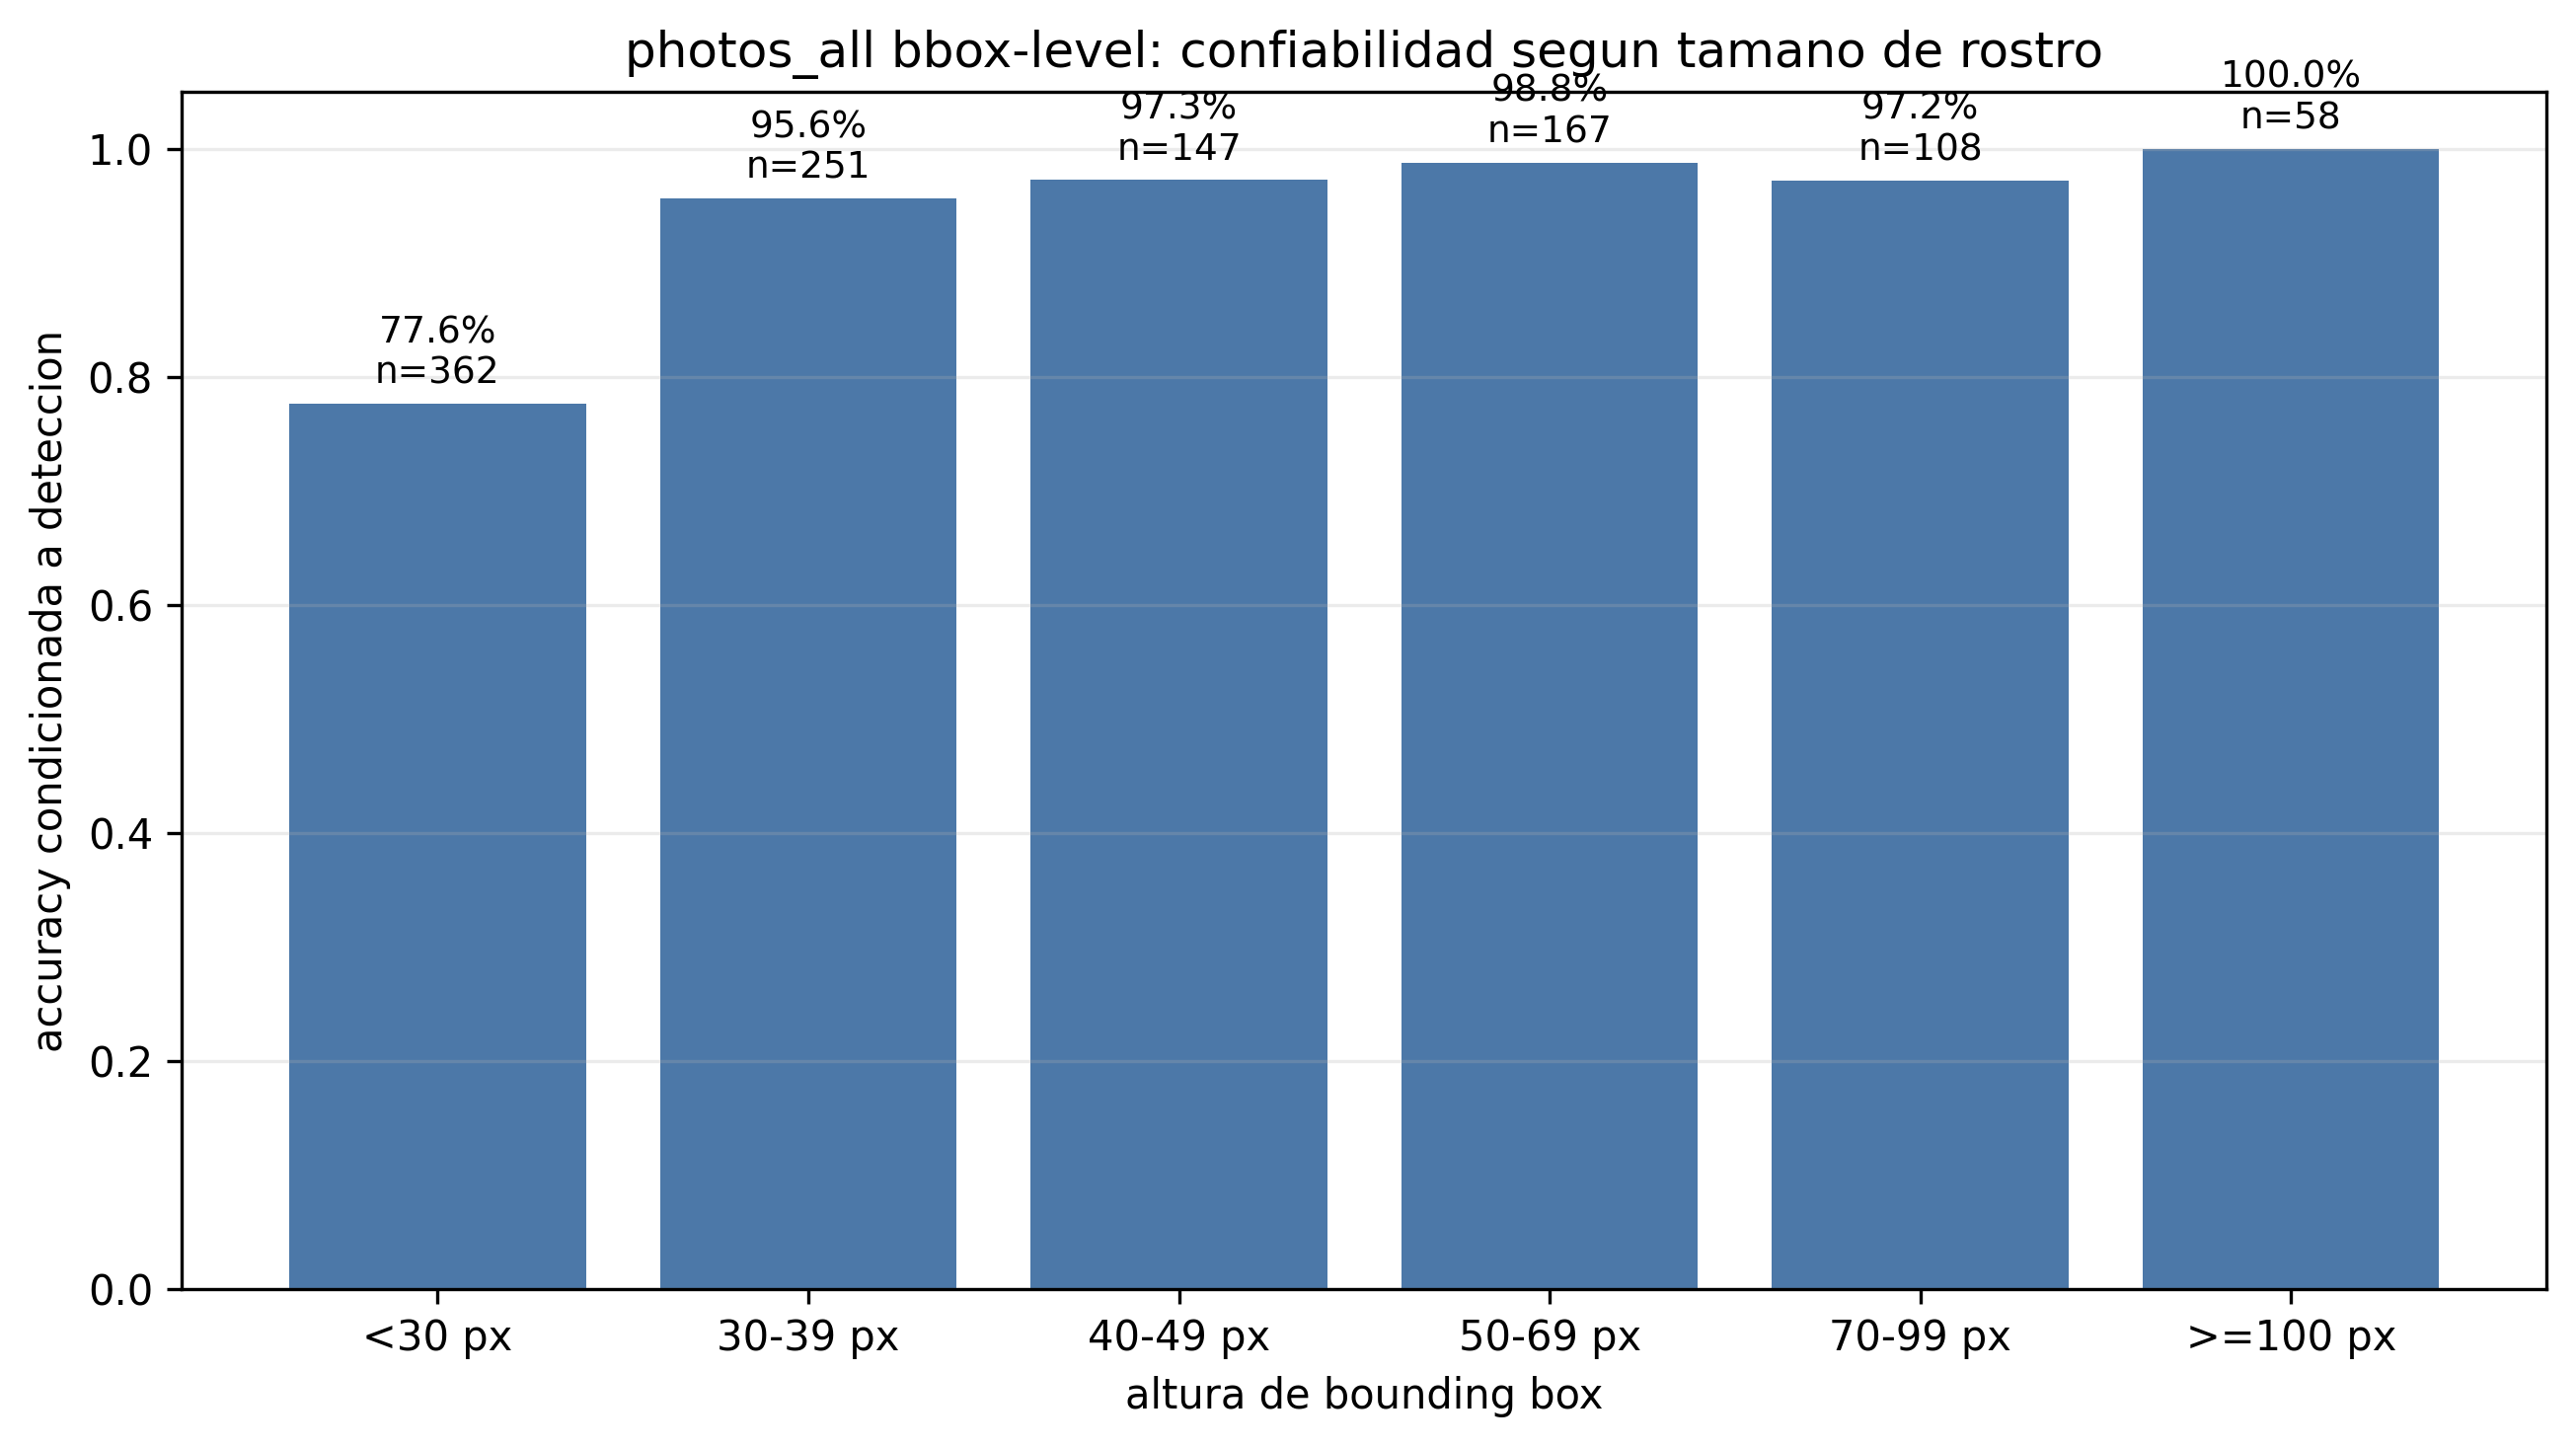
\includegraphics[width=\textwidth]{outputs_v2/figs/metrics/photos_all_bbox_accuracy_by_bbox_height.png}
    \caption{Accuracy condicionada por altura de bbox.}
\end{subfigure}
\hfill
\begin{subfigure}[t]{0.49\textwidth}
    \centering
    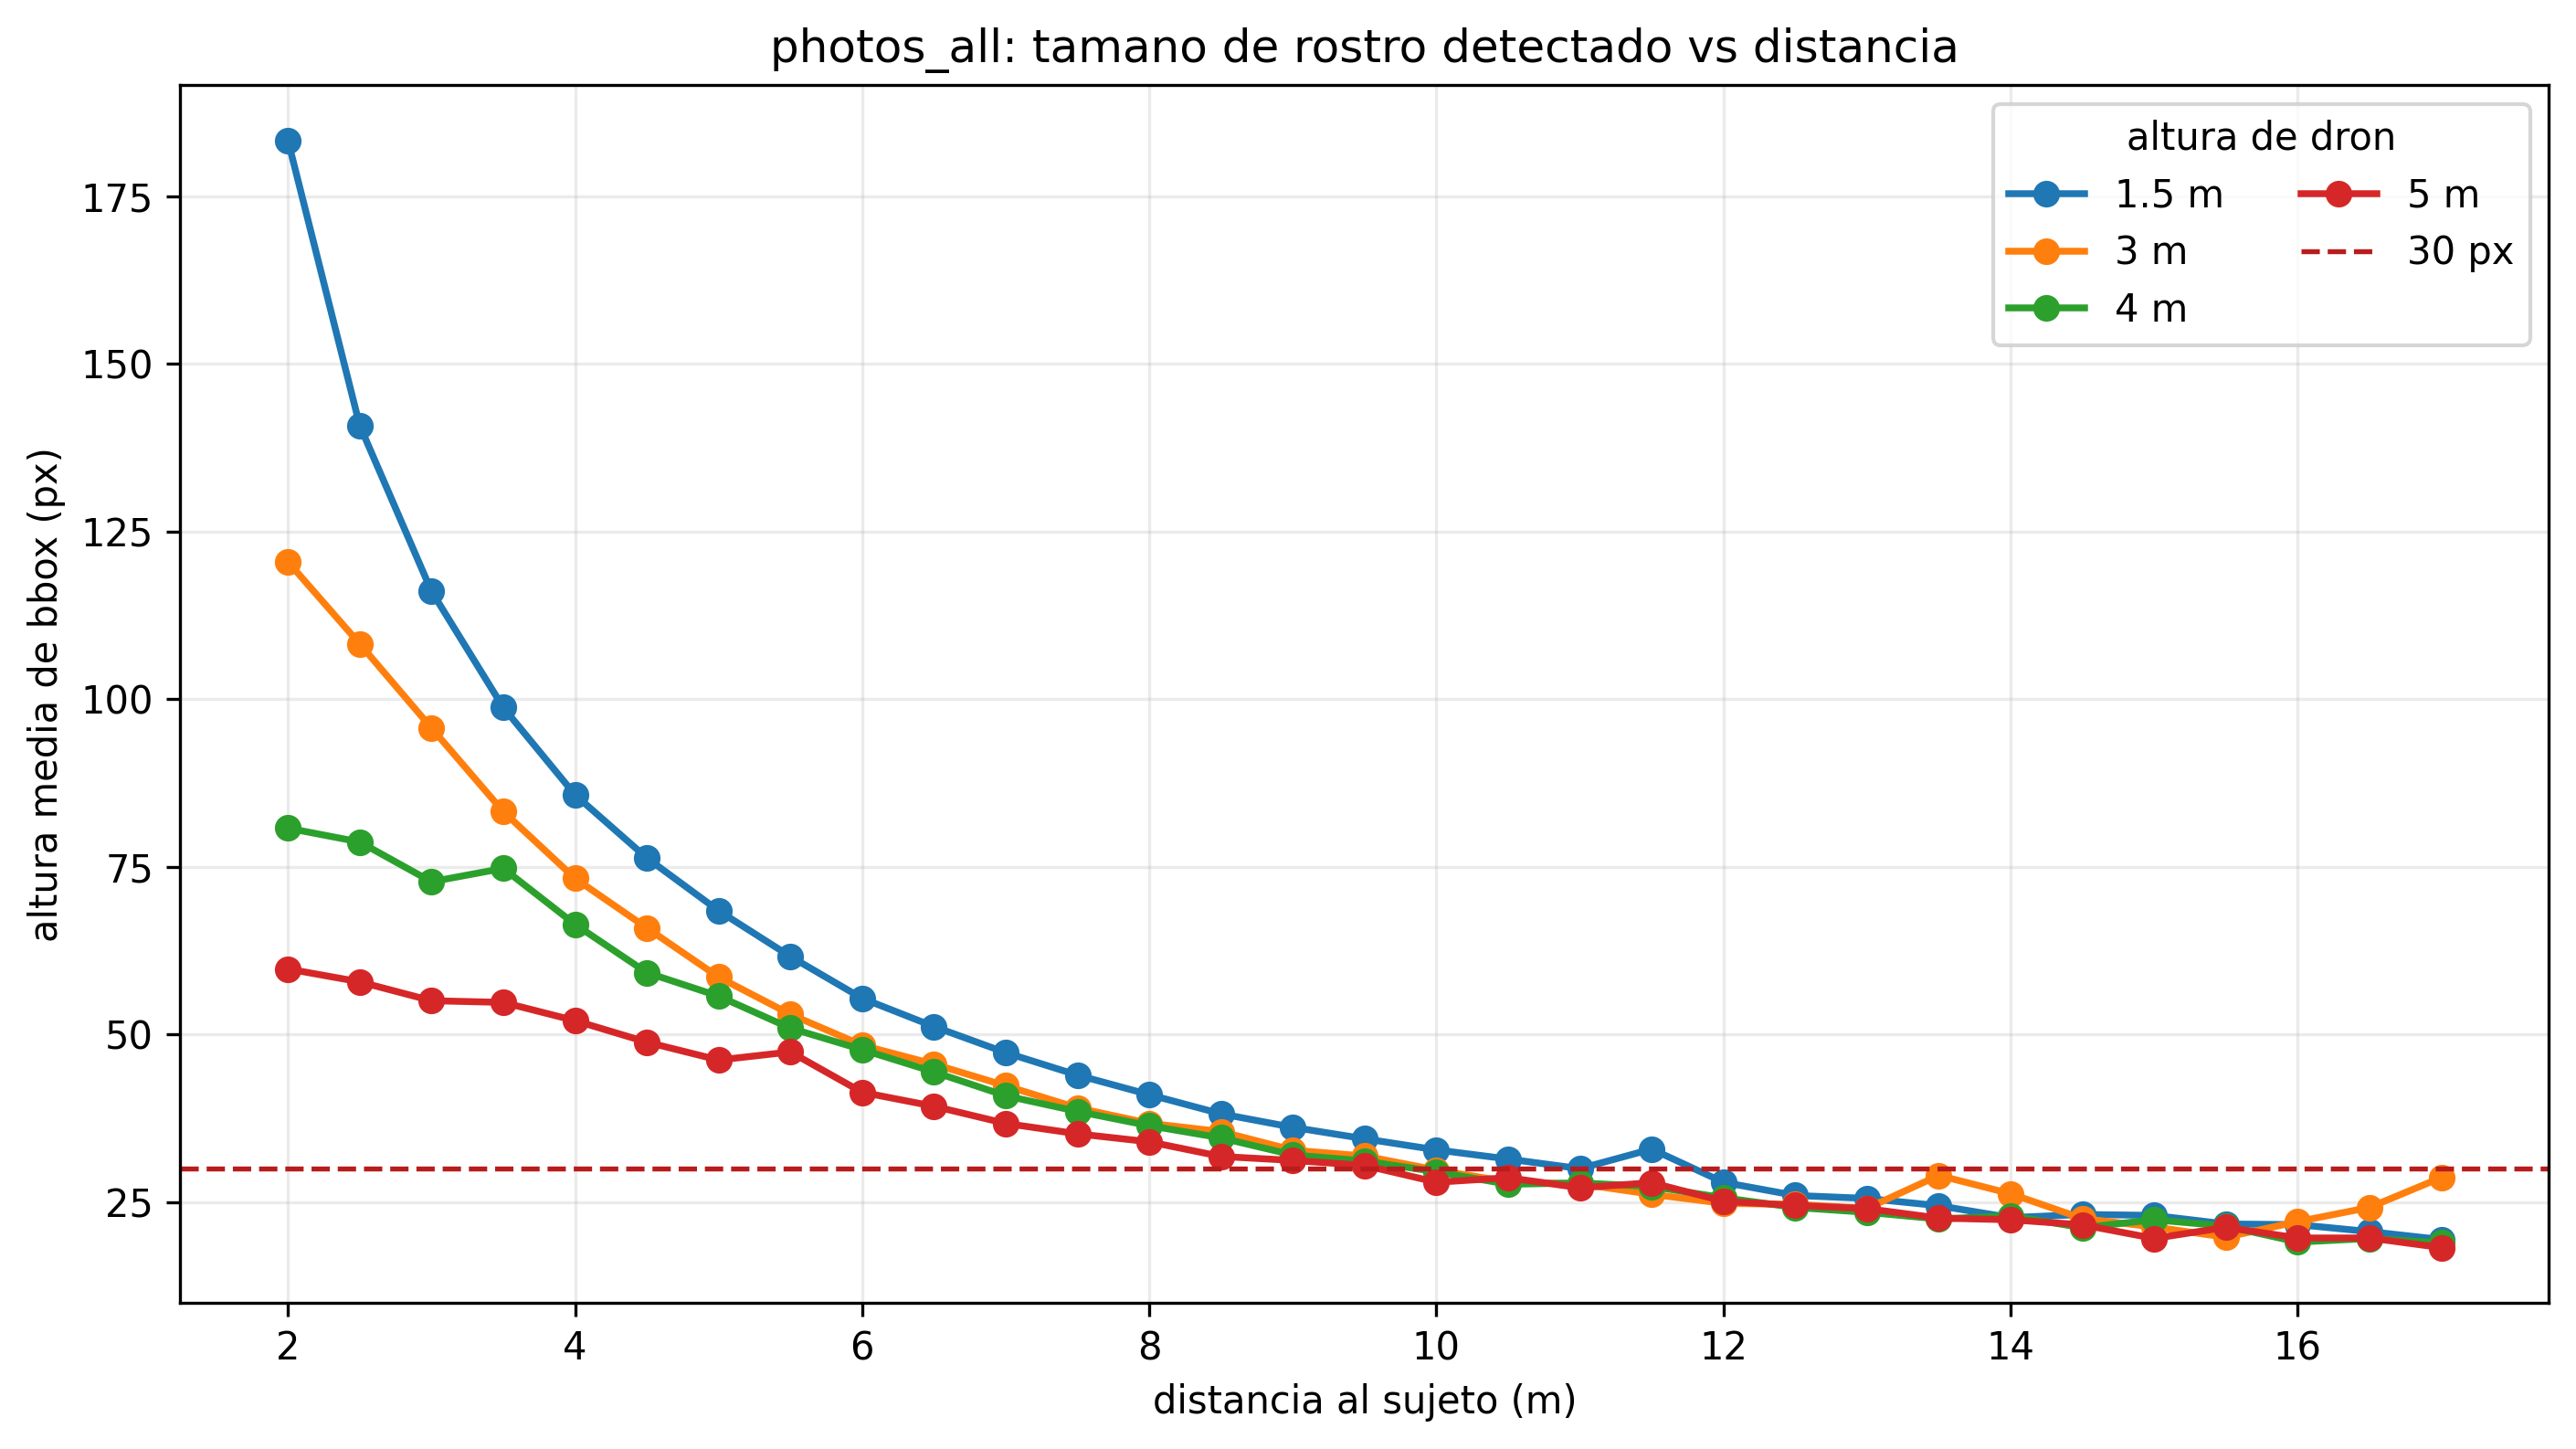
\includegraphics[width=\textwidth]{outputs_v2/figs/metrics/photos_all_bbox_size_vs_distance.png}
    \caption{Altura media de bbox por distancia.}
\end{subfigure}
\caption{Relaci\'on entre tama\~no de rostro detectado, distancia y confiabilidad del reconocimiento.}
\label{fig:bbox_size_reliability}
\end{figure}

Para comparar visualmente con los mapas de Hsu y Chen \cite{hsu2015issues}, se agruparon las distancias en bins de 1.5 m centrados en 2.5, 4.0, 5.5, 7.0, 8.5, 10.0, 11.5, 13.0, 14.5 y 16.0 m. La \autoref{fig:auc_heatmaps} muestra que el AUC en im\'agenes completas se mantiene alto hasta distancias medias y cae con fuerza en el tramo final, mientras que el caso de rostros recortados se conserva alto en casi todo el rango. Esto confirma que \texttt{photos\_all\_faces} sobreestima el rendimiento real del sistema completo.

\begin{figure}[H]
\centering
\begin{subfigure}{0.96\textwidth}
    \centering
    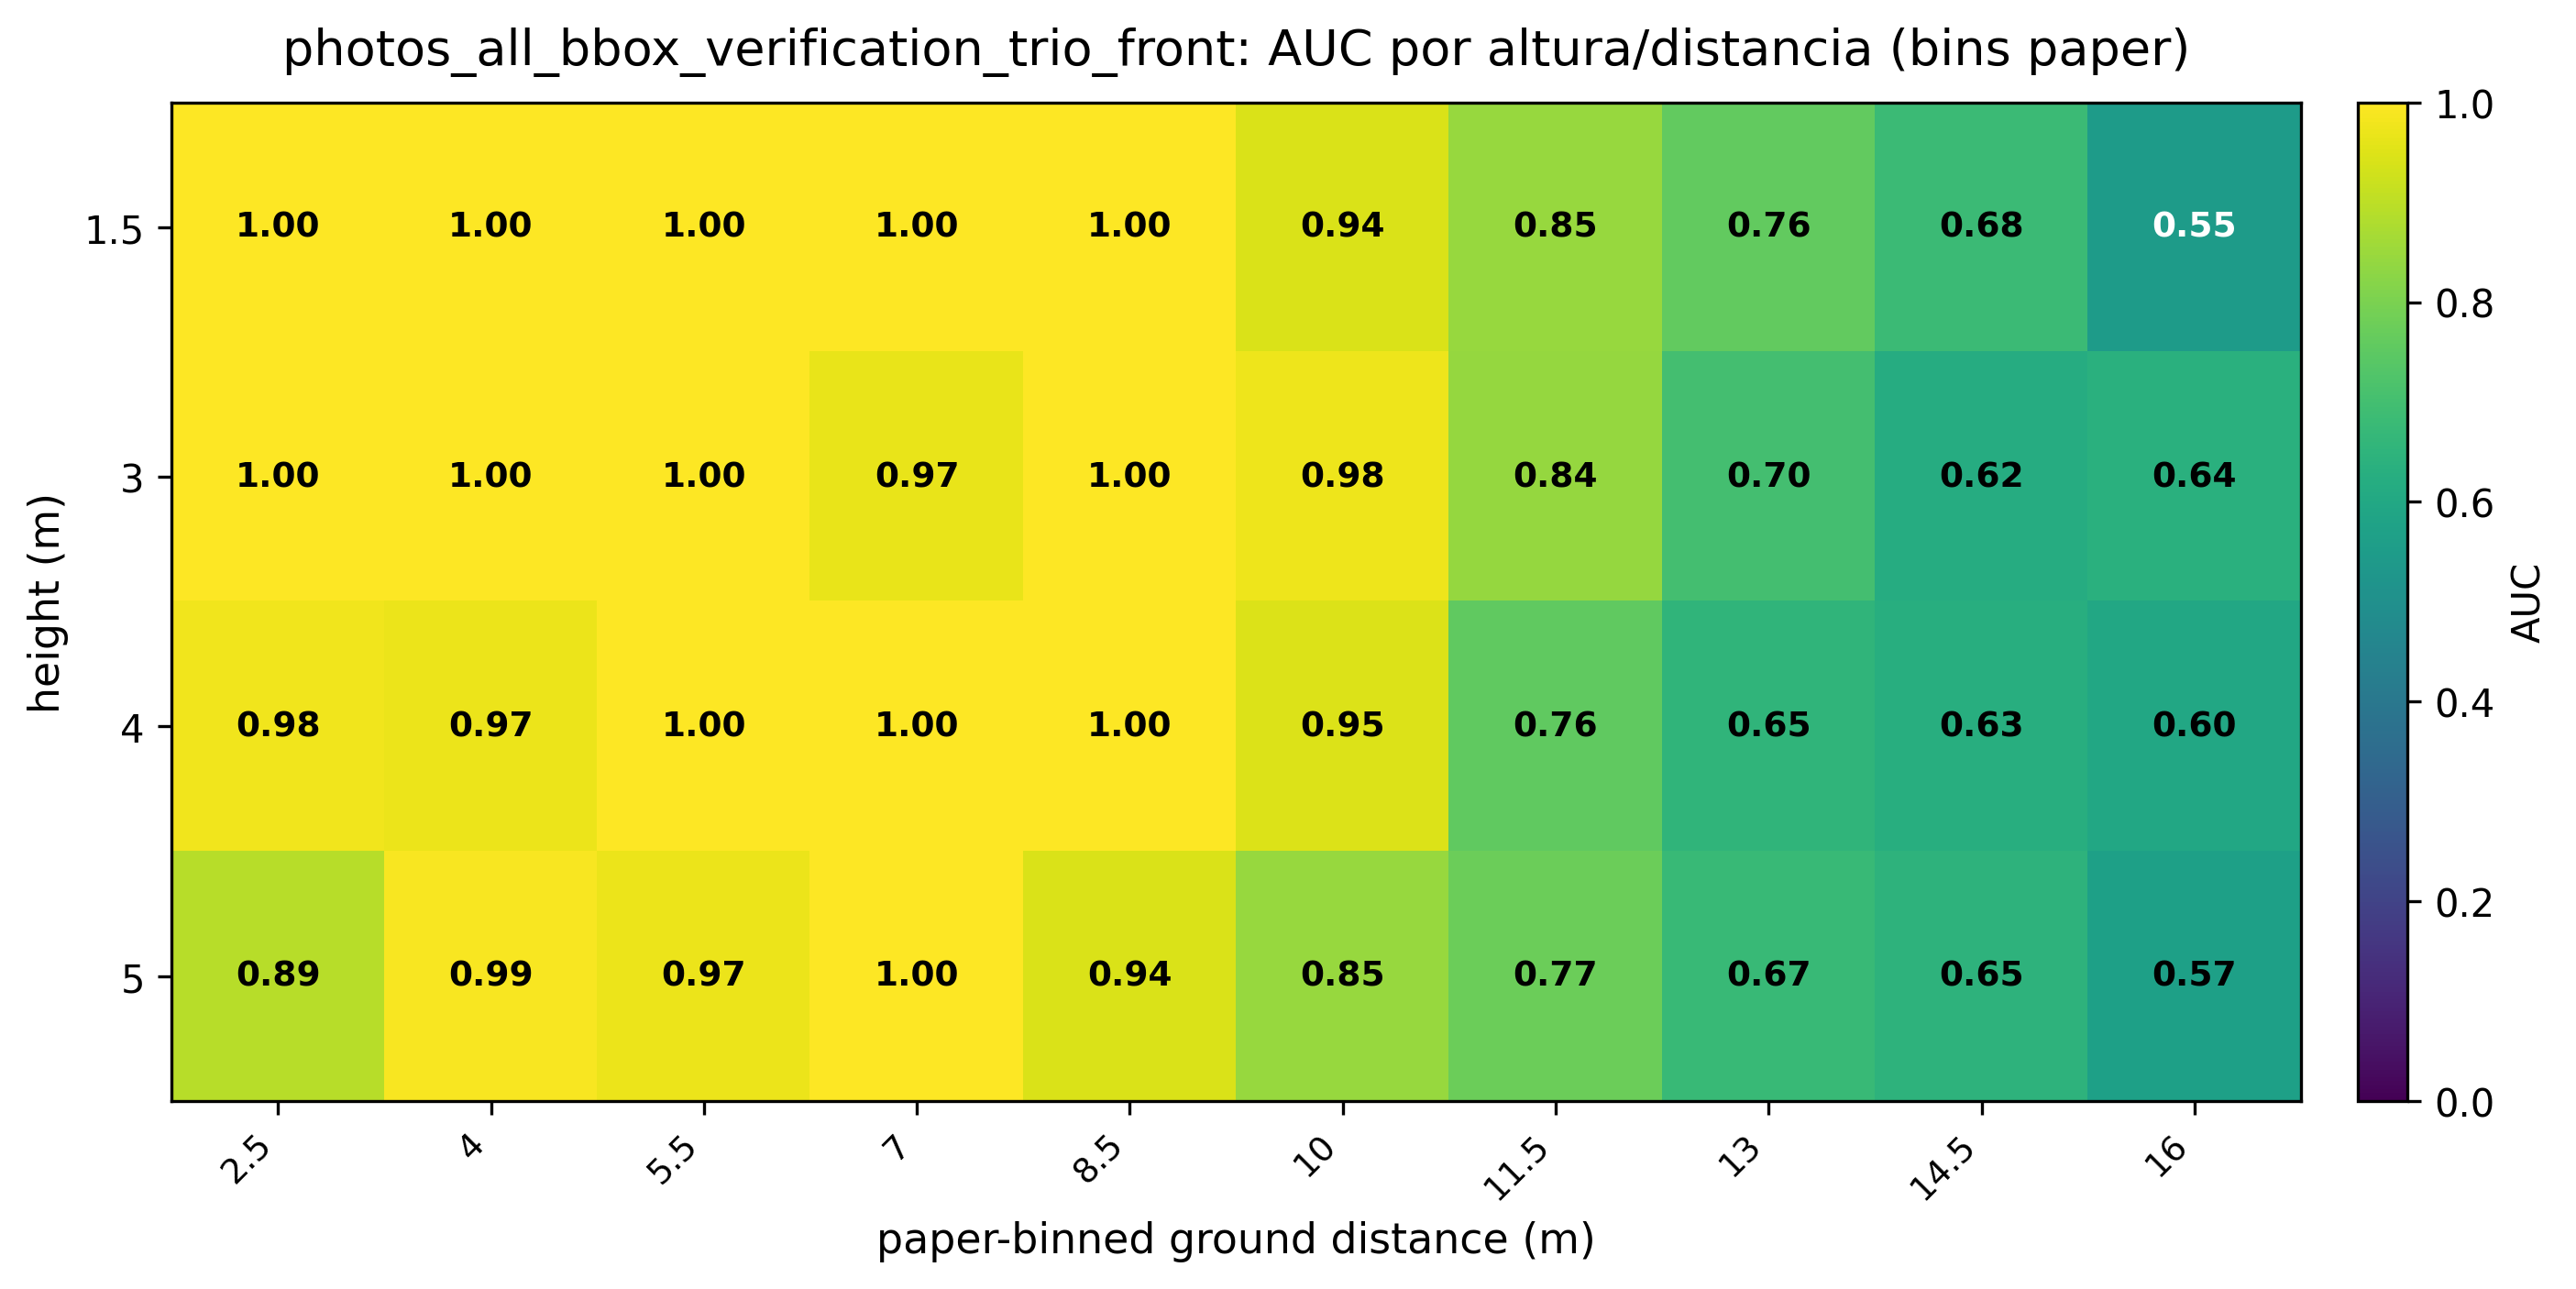
\includegraphics[width=\textwidth]{outputs_v2/figs/metrics/photos_all_bbox_verification_trio_front_auc_paper_height_distance.png}
    \caption{\texttt{photos\_all\_bbox}, end-to-end.}
\end{subfigure}

\vspace{0.4em}

\begin{subfigure}{0.96\textwidth}
    \centering
    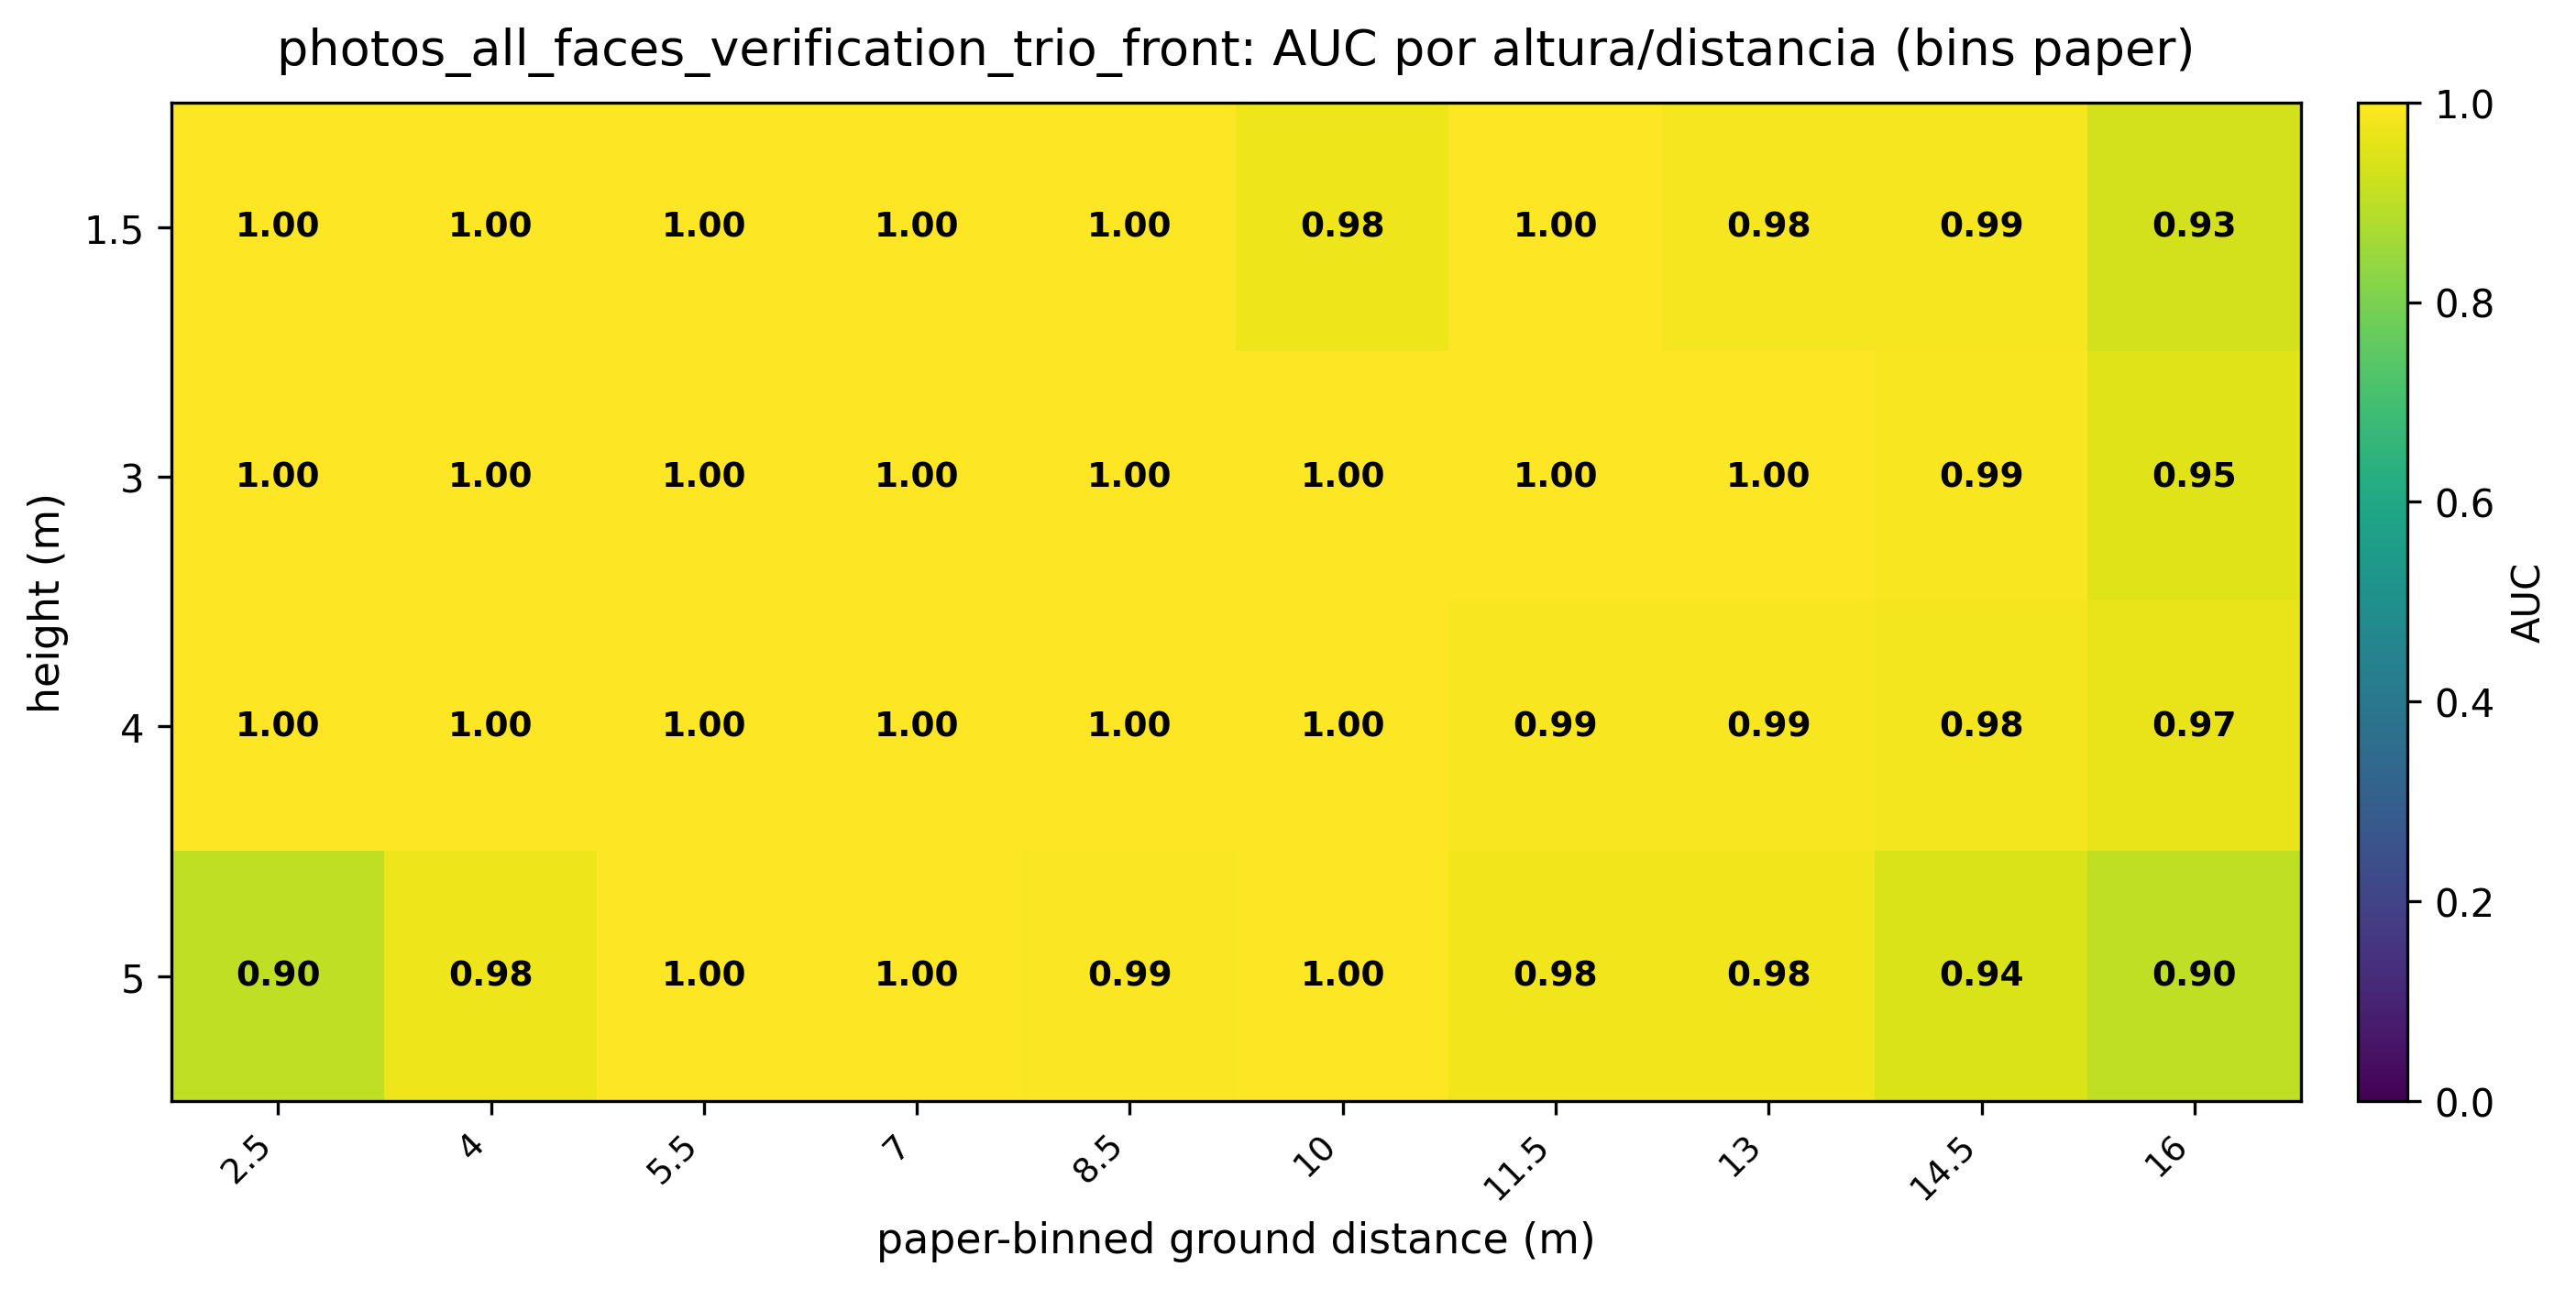
\includegraphics[width=\textwidth]{outputs_v2/figs/metrics/photos_all_faces_verification_trio_front_auc_paper_height_distance.png}
    \caption{\texttt{photos\_all\_faces}.}
\end{subfigure}
\caption{Mapas de calor de AUC por altura y distancia usando bins comparables al paper.}
\label{fig:auc_heatmaps}
\end{figure}

Finalmente, la \autoref{tab:threshold_unknown} reporta la decisi\'on con \texttt{None}/\textit{unknown}. El umbral elegido fue $\tau=0.178772$ desde \texttt{photos\_all\_faces}. Al aplicarlo a \texttt{photos\_all\_bbox}, el sistema obtiene 91.46\% de precisi\'on y 69.87\% de recall. El \texttt{unknown\_rate} sube a 25.25\%, lo que es consistente con un criterio m\'as conservador que evita forzar siempre una identidad entre los 11 sujetos.

\begin{table}[H]
\centering
\caption{M\'etricas con umbral \texttt{None}/\textit{unknown} para \texttt{trio\_front}.}
\label{tab:threshold_unknown}
\begin{adjustbox}{max width=\textwidth}
\begin{tabular}{lccccccc}
\toprule
Conjunto & Umbral & TP & FP & FN & Precisi\'on & Recall & F1 \\
\midrule
\texttt{photos\_all\_faces} & 0.178772 & 1221 & 8 & 143 & 99.35\% & 89.52\% & 94.18\% \\
\texttt{photos\_all\_bbox} & 0.178772 & 953 & 89 & 411 & 91.46\% & 69.87\% & 79.22\% \\
\bottomrule
\end{tabular}
\end{adjustbox}
\end{table}

\subsection{Comparaci\'on con V1 del proyecto}

La versi\'on V1 del proyecto usaba \texttt{portraits} como galer\'ia principal. En la copia local, esa carpeta solo contiene referencias para 7 de los 11 sujetos; por lo tanto, V1 eval\'ua 868 probes en el Experimento A y deja 496 probes fuera por no tener galer\'ia. La versi\'on V2 corrige este punto al construir galer\'ias desde \texttt{trio\_cam} y \texttt{trio\_gp}, cubriendo los 11 sujetos y evaluando los 1364 recortes disponibles.

\begin{table}[H]
\centering
\caption{Comparaci\'on entre V1 y V2 en rostros recortados.}
\label{tab:v1_v2_faces}
\begin{adjustbox}{max width=\textwidth}
\begin{tabular}{lcccccc}
\toprule
Versi\'on & Galer\'ia & Sujetos & Probes evaluados & Detectados & Correctos & \accglobal{} \\
\midrule
V1 & \texttt{portraits} & 7 & 868 & 862 & 788 & 90.78\% \\
V2 & \texttt{trio\_front} & 11 & 1364 & 1350 & 1316 & 96.48\% \\
\bottomrule
\end{tabular}
\end{adjustbox}
\end{table}

La mejora de V2 en la \autoref{tab:v1_v2_faces} no proviene de entrenar ArcFace, sino de una galer\'ia m\'as completa y compatible con el protocolo. La tasa de detecci\'on se mantiene muy alta en ambas versiones (99.31\% en V1 y 98.97\% en V2), pero la exactitud global sube de 90.78\% a 96.48\% y el n\'umero de aciertos aumenta de 788 a 1316 porque ahora se eval\'uan todos los sujetos.

En im\'agenes completas, el recall global de identidades esperadas queda parecido entre V1 y V2, pero el denominador cambia de forma importante. V1 recupera 684 de 868 identidades esperadas con galer\'ia; V2 recupera 1070 de 1364. Es decir, V2 mantiene pr\'acticamente el mismo recall mientras cubre todos los sujetos y elimina las identidades sin referencia.

\begin{table}[H]
\centering
\caption{Comparaci\'on entre V1 y V2 en im\'agenes completas.}
\label{tab:v1_v2_full}
\begin{adjustbox}{max width=\textwidth}
\begin{tabular}{lcccccc}
\toprule
Versi\'on & Esperadas con galer\'ia & Recuperadas & Sin galer\'ia & Inesperadas & Jaccard medio & Recall global \\
\midrule
V1 & 868 & 684 & 496 & 399 & 54.10\% & 78.80\% \\
V2 & 1364 & 1070 & 0 & 42 & 77.22\% & 78.45\% \\
\bottomrule
\end{tabular}
\end{adjustbox}
\end{table}

La \autoref{tab:v1_v2_full} muestra la mejora metodol\'ogica m\'as importante de V2. Aunque el recall global baja levemente de 78.80\% a 78.45\%, ahora se mide sobre todos los sujetos. Adem\'as, las identidades inesperadas bajan de 399 a 42 y la similitud de Jaccard media sube de 54.10\% a 77.22\%. Esto indica que V2 no solo encuentra identidades esperadas, sino que tambi\'en predice conjuntos mucho m\'as coherentes con la etiqueta de cada imagen.

\section{Discusi\'on}
\label{sec:discusion}

\subsection{Comparaci\'on con trabajos previos}
\label{sec:comparacion_previos}

El paper de Hsu y Chen \cite{hsu2015issues} estudia un escenario estrechamente relacionado: 620 im\'agenes y 1364 rostros objetivo capturados con una configuraci\'on tipo dron, variando altura, distancia y \'angulo de depresi\'on. La diferencia principal es tecnol\'ogica y metodol\'ogica: el paper eval\'ua Face++, ReKognition y detectores cl\'asicos Haar/LBP, mientras que este proyecto usa InsightFace/ArcFace y reporta recuperaci\'on de identidades, m\'etricas \textit{bbox-level} y AUC por verificaci\'on. Un trabajo posterior tambi\'en estudia detecci\'on y reconocimiento con aprendizaje profundo sobre DroneFace \cite{rostami2022deep}; en este informe se usa como referencia de contexto moderno, pero no como comparaci\'on num\'erica principal porque el protocolo local no replica su entrenamiento ni sus particiones.

La \autoref{tab:paper_detection} compara resultados de detecci\'on. Esta comparaci\'on debe leerse con cautela porque las unidades no son id\'enticas: Hsu y Chen reportan TPR/FPR por rostro objetivo, mientras que el Experimento B reporta detecci\'on por imagen y el an\'alisis \textit{bbox-level} permite estimar cobertura por slot esperado. Aun as\'i, el resultado muestra que la detecci\'on directa de servicios comerciales en el paper era limitada, mientras que el flujo V2 cubre 80.13\% de los slots esperados antes de exigir identidad correcta.

\begin{table}[H]
\centering
\caption{Detecci\'on facial: trabajos previos versus resultados del proyecto.}
\label{tab:paper_detection}
\begin{adjustbox}{max width=\textwidth}
\begin{tabular}{lcccc}
\toprule
Fuente & M\'etodo & Unidad & M\'etrica de detecci\'on & Valor \\
\midrule
Hsu y Chen \cite{hsu2015issues} & Face++ directo & Rostros objetivo & TPR & 14.00\% \\
Hsu y Chen \cite{hsu2015issues} & ReKognition directo & Rostros objetivo & TPR & 27.00\% \\
Hsu y Chen \cite{hsu2015issues} & Haar alt & Rostros objetivo & TPR / FPR & 77.00\% / 37.00\% \\
Hsu y Chen \cite{hsu2015issues} & Haar alt2 & Rostros objetivo & TPR / FPR & 78.00\% / 57.00\% \\
Proyecto V2 & InsightFace, imagen completa & Imagen & Al menos una detecci\'on & 91.45\% \\
Proyecto V2 & InsightFace, orden espacial & Slot esperado & Detecci\'on en slot & 80.13\% \\
\bottomrule
\end{tabular}
\end{adjustbox}
\end{table}

La \autoref{tab:paper_recognition} resume la comparaci\'on de reconocimiento. En rostros ya detectados, el proyecto obtiene AUC \textit{detected-only} de 0.953 en \texttt{photos\_all\_bbox}, lo que sugiere una etapa de reconocimiento competitiva. Sin embargo, la comparaci\'on m\'as justa para sistema completo es el AUC end-to-end de 0.822, mostrado tambi\'en en la \autoref{fig:roc_bbox}. Este valor es menor que la lectura optimista de rostros recortados y refleja el costo de las caras no detectadas.

\begin{table}[H]
\centering
\caption{Reconocimiento: lectura comparativa entre Hsu y Chen y V2.}
\label{tab:paper_recognition}
\begin{adjustbox}{max width=\textwidth}
\begin{tabular}{llll}
\toprule
Fuente & M\'etodo & M\'etrica reportada & Lectura comparable \\
\midrule
Hsu y Chen \cite{hsu2015issues} & Face++ & AUC/score & Distinguible hasta cerca de 12 m \\
Hsu y Chen \cite{hsu2015issues} & ReKognition & AUC/score & Distinguible hasta cerca de 14 m \\
Proyecto V2 & InsightFace/ArcFace & AUC end-to-end & 0.822 en \texttt{photos\_all\_bbox} \\
Proyecto V2 & InsightFace/ArcFace & AUC detected-only & 0.953 en \texttt{photos\_all\_bbox} \\
Proyecto V2 & InsightFace/ArcFace & \accglobal{} en recortes & 96.48\% global \\
\bottomrule
\end{tabular}
\end{adjustbox}
\end{table}

\subsection{Interpretaci\'on general}
\label{sec:interpretacion_general}

Los resultados muestran que el reconocimiento sobre rostros recortados es robusto en esta configuraci\'on. Con la galer\'ia \texttt{trio\_front}, el Experimento A alcanza 96.48\% de \accglobal{} sobre los 1364 probes. Este valor es superior al baseline preliminar con \texttt{portraits}, que evaluaba menos sujetos por falta de galer\'ia. La mejora no implica que el modelo haya aprendido nuevas representaciones; se debe a una galer\'ia m\'as completa y m\'as adecuada al protocolo.

La diferencia entre los Experimentos A y B es relevante. Pasar desde un rostro recortado a una imagen completa reduce la m\'etrica principal desde 96.48\% a 78.45\%. Esta ca\'ida confirma que el cuello de botella no es solamente la comparaci\'on de embeddings: tambi\'en influyen la detecci\'on de rostros peque\~nos, el alineamiento, la escala y la calidad visual de la caja detectada.

El Experimento C refuerza esta interpretaci\'on. Cuando se exige coherencia a nivel de caja y posici\'on espacial, el F1 global queda en 79.77\%. La precisi\'on de 88.33\% es mayor que el recall de 72.73\%, por lo que el sistema tiende a cometer m\'as omisiones que identificaciones inesperadas. La \autoref{tab:detection_recognition_split} separa este efecto: el detector cubre 80.13\% de los slots esperados, mientras que el reconocimiento condicionado a detecci\'on alcanza 90.76\%. Esto es consistente con la diferencia entre el AUC end-to-end de 0.822 y el AUC \textit{detected-only} de 0.953 reportados en la \autoref{tab:verification_auc}.

La comparaci\'on de galer\'ias tambi\'en entrega una conclusi\'on clara. \texttt{trio\_front} fue la mejor galer\'ia en los tres protocolos, aunque \texttt{trio\_all} qued\'o muy cerca. Agregar vistas laterales no mejor\'o el resultado final; posiblemente el promedio multi-pose introduce variabilidad que no siempre coincide con los probes evaluados. En este dataset, las referencias frontales parecen representar mejor los rostros observados en \texttt{photos\_all\_faces} y \texttt{photos\_all}.

Frente a V1, V2 debe entenderse como una versi\'on metodol\'ogicamente m\'as completa. La comparaci\'on m\'as relevante no es solo 90.78\% contra 96.48\% en recortes, sino el hecho de que V2 eval\'ua los 11 sujetos y reduce las predicciones inesperadas en im\'agenes completas.

\subsection{S\'intesis comparativa con trabajos previos}
\label{sec:discusion_comparativa}

La \autoref{fig:auc_heatmaps} permite comparar tendencias por altura y distancia. En V2, la condici\'on end-to-end conserva buen AUC en distancias cortas y medias, pero se debilita en el tramo final. En el paper, ReKognition con pre-detecci\'on parece mantenerse fuerte en varias zonas hasta distancias medias-altas \cite{hsu2015issues}. Por lo tanto, no corresponde afirmar que el proyecto supera globalmente al paper. Lo correcto es que V2 mejora la reproducibilidad local y la separaci\'on de m\'etricas, mientras que el paper tiene una evaluaci\'on m\'as dise\~nada para comparar servicios y estudiar l\'imites por distancia/altura.

\begin{table}[H]
\centering
\caption{Discusi\'on comparativa: fortalezas relativas y cautelas de interpretaci\'on.}
\label{tab:comparative_discussion}
{\small
\setlength{\tabcolsep}{4pt}
\renewcommand{\arraystretch}{1.15}
\begin{adjustbox}{max width=\textwidth}
\begin{tabular}{>{\raggedright\arraybackslash}p{0.16\textwidth}
                >{\raggedright\arraybackslash}p{0.27\textwidth}
                >{\raggedright\arraybackslash}p{0.27\textwidth}
                >{\raggedright\arraybackslash}p{0.22\textwidth}}
\toprule
Aspecto & Hsu y Chen & Proyecto V2 & Lectura \\
\midrule
Detecci\'on directa & TPR/FPR para Face++, ReKognition y Haar/LBP. & Detecci\'on por imagen y por slot espacial. & Unidades distintas; lectura cautelosa. \\
Reconocimiento con rostro detectado & ReKognition se mantiene fuerte en zonas medias-altas. & AUC detected-only = 0.953 en \texttt{photos\_all\_bbox}. & V2 es fuerte cuando detecta la cara. \\
Sistema end-to-end & Eval\'ua servicios y pre-detecci\'on como flujo completo. & AUC end-to-end = 0.822; F1 bbox-level = 79.77\%. & Comparaci\'on m\'as justa, no superioridad global. \\
Robustez a distancia & Protocolo centrado en distancia, altura y \'angulo. & Ca\'ida en distancias largas; umbral pr\'actico de 30 px. & Ambos apuntan a escala/distancia. \\
Control local & APIs externas de 2015. & Modelo local preentrenado y pipeline reproducible. & V2 gana en control experimental. \\
Anotaciones & Protocolo dise\~nado para el paper. & Orden espacial manual por prefijo. & \'Util, pero limitado. \\
\bottomrule
\end{tabular}
\end{adjustbox}
}
\end{table}

La lectura de la \autoref{tab:comparative_discussion} es mixta. Hsu y Chen ganan en comparaci\'on directa entre servicios y en dise\~no experimental orientado a medir l\'imites de distancia/altura. El proyecto V2 gana en reproducibilidad local, cobertura de los 11 sujetos, evaluaci\'on \textit{bbox-level} con TP/FP/FN/F1 y separaci\'on entre detecci\'on, reconocimiento condicionado y desempe\~no end-to-end. La conclusi\'on equilibrada es que V2 es competitivo y m\'as moderno, pero no debe presentarse como superior al paper en todas las condiciones.

\subsection{Limitaciones}

La evaluaci\'on sigue siendo limitada por la disponibilidad de anotaciones. En \texttt{photos\_all}, las etiquetas originales indican conjuntos de sujetos, no identidades por caja. El Experimento C aproxima esta evaluaci\'on usando orden espacial manual por prefijo, pero no reemplaza una anotaci\'on exhaustiva de cada bounding box en cada imagen.

El sistema principal opera en modo \textit{closed-set}; el an\'alisis con \texttt{None}/\textit{unknown} de la \autoref{tab:threshold_unknown} es una extensi\'on por umbral, no una evaluaci\'on \textit{open-set} completa con sujetos externos a la galer\'ia. En un sistema real, ser\'ia necesario medir con distractores que no pertenezcan a los 11 sujetos de DroneFace para estimar rechazos correctos, falsas aceptaciones y falsos rechazos frente a personas desconocidas. Adem\'as, no se hizo \textit{fine-tuning} de ArcFace sobre DroneFace, no se evalu\'o tiempo real y no se integr\'o control de dron.

\section{Conclusiones}
\label{sec:conclusiones}

Se implement\'o y evalu\'o un pipeline reproducible de reconocimiento facial desde im\'agenes de dron usando DroneFace e InsightFace/ArcFace preentrenado. La versi\'on final construye galer\'ias desde \texttt{trio\_cam} y \texttt{trio\_gp}, lo que permite cubrir los 11 sujetos del dataset.

Los resultados principales son:

\begin{itemize}
    \item En rostros recortados, \texttt{trio\_front} obtuvo 96.48\% de \accglobal{}.
    \item En im\'agenes completas, \texttt{trio\_front} recuper\'o 78.45\% de las identidades esperadas.
    \item En evaluaci\'on \textit{bbox-level}, \texttt{trio\_front} alcanz\'o F1 de 79.77\%, con 88.33\% de precisi\'on y 72.73\% de recall.
    \item En verificaci\'on, \texttt{photos\_all\_bbox} obtuvo AUC end-to-end de 0.822 y AUC \textit{detected-only} de 0.953.
    \item Condicionado a detecci\'on, el reconocimiento cay\'o a 77.62\% cuando la altura de la caja fue menor a 30 px; desde 30 px, todos los bins quedaron sobre 95\%.
    \item Respecto de V1, V2 ampl\'ia la evaluaci\'on de 7 a 11 sujetos, elimina 496 identidades sin galer\'ia y reduce las identidades inesperadas de 399 a 42 en im\'agenes completas.
\end{itemize}

El aprendizaje principal es que el reconocimiento facial desde drones no puede evaluarse solamente sobre recortes. El pipeline completo pierde desempe\~no cuando debe detectar rostros peque\~nos en la imagen completa, mientras que el reconocimiento condicionado a detecci\'on es bastante m\'as fuerte. Como trabajo futuro, se recomienda etiquetar manualmente cada bounding box con identidad, evaluar un protocolo \textit{open-set} con distractores, estudiar umbrales de similitud y comparar ArcFace con otros modelos o estrategias de adaptaci\'on al dominio.

\newpage
\phantomsection
\addcontentsline{toc}{section}{Referencias}
\bibliographystyle{ieeetr}
\bibliography{referencias}

\end{document}
